%%%--- Template for master thesis at SfS
%%%--- Modified template with more comments and examples -- SG, 11/06/09
%%%------
\documentclass[11pt,a4paper,twoside,openright]{report}
%%not needed \usepackage{E}
\usepackage[english]{ETHDAsfs}%--> ETHDASA + fancyheadings + ... "umlaute" 
%  + sfs-hyper -> hyperref 

\usepackage{amsbsy}%% for \boldsymbol and \pmb{.}
\usepackage{amssymb}%% calls  amsfonts...
%or \usepackage{german8}%-- =  german  +  isolatin1
\usepackage{graphicx}%-- f�r PostScript-Grafiken (besser als  psfig!)
%\usepackage[draft]{graphicx} % grafics shown as boxes --> faster compilation
%
\usepackage[longnamesfirst]{natbib}%was {sfsbib}%- F�r  Literatur-Referenzen
%           ^^^^^^^^^^^^^^ 1) "Hampel, Ronchetti, ..,"  2) "Hampel et al"
% Engineers (and other funny people) want to see [1], [2] 
% ---> use 'numbers' : \usepackage[longnamesfirst,number]{natbib}
%
%
\usepackage{texab}%- 'tex Abk�rzungen' /u/sfs/tex/tex/latex/texab.sty
        %%- z.B.  \R, \Z, \Q, \Nat f�r reelle, ganze, rationale, nat�rl. Zahlen;
        %%-       \N   (Normalvert.)  \W == Wahrscheinlichkeit .....
        %%-  \med, \var, \Cov, \....
        %%-  \abs{x} == |x|   und   \norm{y} ==  || y ||   (aber anst�ndig)
%% NOTE: texab contains many useful definitions and "shortcuts". It is
%% worth to open the file and have a look at them. HOWEVER, some
%% definitions are a bit can lead to conflicts with other packages. You
%% might for example want to comment out the line defininf \IF as an
%% operator when working with the algorithmic package, or to comment out
%% the line defining a command \Cite with working with the Biblatex package  
\usepackage{amsmath}
%\usepackage{mathrsfs}% Raph Smith's Formal Script font --> provides \mathscr
\usepackage{enumerate}% Fuer selbstdefinierte Nummerierungen
%--------
\usepackage{relsize}%-> \smaller (etc) used here
\usepackage{color} %% to allow cloring in code listings
\definecolor{Mygrey}{gray}{0.75}
\usepackage{listings}% Fuer R-code, C-code, ....  and settings for these:
\lstloadlanguages{R}
\lstset{ %% Hilfe unter z.B. http://en.wikibooks.org/wiki/LaTeX/Packages/Listings
language=R,
basicstyle=\scriptsize\ttfamily,
commentstyle=\ttfamily\color{Mygrey},
numbers=left,
numberstyle=\ttfamily\color{Mygrey}\footnotesize,
stepnumber=1,
numbersep=5pt,
backgroundcolor=\color{white},
showspaces=false,
showstringspaces=false,
showtabs=false,
frame=single,
tabsize=2,
captionpos=b,
breaklines=true,
%breakatwhitespace=false,
keywordstyle={},
morekeywords={},
xleftmargin=4ex, 
literate={<-}{{$\leftarrow$}}1 {~}{{$\sim$}}1}
\lstset{escapeinside={(*}{*)}} % for (*\ref{ }*) inside lstlistings (Scode) 
%%----------------------------------------------------------------------------

%%------- Theoreme ---
\newtheorem{definition}{Definition}[subsection]
\newtheorem{lemma}[definition]{Lemma}
\newtheorem{theorem}[definition]{Theorem}
\newtheorem{Coro}[definition]{Corollary}
\theoremstyle{definition} 
\newtheorem{example}[definition]{Example}
\newtheorem*{note}{Note}
\newtheorem*{remark}{Remark}

\DeclareMathOperator*{\plim}{plim}
% \def\MR#1{\href{http://www.ams.org/mathscinet-getitem?mr=#1}{MR#1}}

% \newcommand{\Lecture}[3]{\marginpar{#3.#2.#1}}
% \newcommand{\Fu}{\mathcal{F}}
\newcommand{\aatop}[2]{\genfrac{}{}{0pt}{}{#1}{#2}}

%\renewcommand{\theequation}{\arabic{equation}}
\numberwithin{equation}{subsection}

%%%%%%%%%%%%%%%%%%%%%%%%%%%%%%%%%%%%%%%%%%%%%%%%%
%%% Path for your figures                      %%%
%%%%%%%%%%%%%%%%%%%%%%%%%%%%%%%%%%%%%%%%%%%%%%%%%
% Set the paths where all figures are taken from:
\graphicspath{{Pictures/}}

%%%%%%%%%%%%%%%%%%%%%%%%%%%%%%%%%%%%%%%%%%%%%%%%%
%%% Define your own commands here             %%%
%%%%%%%%%%%%%%%%%%%%%%%%%%%%%%%%%%%%%%%%%%%%%%%%%
\newcommand{\Bruch}[2]{{}^{#1}\!\!/\!_{#2}}
\renewcommand{\labelenumi}{\roman{enumi}.)}



\begin{document}
\bibliographystyle{chicago}% ---> Hampel,F., E.Ronchetti,... W.Stahel(1986) ...
 %was \bibliographystyle{sfsbib}\citationstyle{dcu} %OR DEFAULT : \citationstyle{agsm}

\pagenumbering{roman}%- roman numbering for first few pages

%%%%%%%%%%%%%%%%%%%%%%%%%%%%%%%%%%%%%%%%%%%%%%%%%
%%% Title page                                %%%
%%%%%%%%%%%%%%%%%%%%%%%%%%%%%%%%%%%%%%%%%%%%%%%%%
\period{Summer 2009}
\dasatype{Master Thesis}
\students{Student Muster}
\mainreaderprefix{Adviser:}
\mainreader{Prof.\ Dr.\ Sara van de Geer}
\alternatereaderprefix{Co-Adviser}
\alternatereader{Markus Kalisch}
\submissiondate{August 19th 2009}
\title{The title of my thesis \\ which should be split on \\ several lines
  if it is too long}

\maketitle%- Titelseite wird abgeschlossen
\cleardoublepage
 %%~~~~~~~~~~~~~~~~~~~~~~~~~~~~~~~~~~~~~~~~

%%%%%%%%%%%%%%%%%%%%%%%%%%%%%%%%%%%%%%%%%%%%%%%%%
%%% Insert here acknowledgements and abstract %%%
%%%%%%%%%%%%%%%%%%%%%%%%%%%%%%%%%%%%%%%%%%%%%%%%%
%% Dedication (optional)
\markright{}
\vspace*{\stretch{1}}
\begin{center}
    To some special person
\end{center}
\vspace*{\stretch{2}}

% Preface (optional)
\newpage
\markboth{Preface}{Preface}
\include{Preface}

% Abstract should not be longer than one page.
\newpage
\markboth{Abstract}{Abstract}
\chapter*{Abstract}

Systems that work in a repetitive manner use Iterative Learning Control (ILC) algorithms to iteratively improve the performance over a given repeated task or trajectory. The feed-forward control signal is modified in each iteration to reduce the error or the deviation from the given reference trajectory. The limitation with ILC is that it assumes the task or the trajectory to be fixed over iterations. ILC cannot handle the cases when the trajectory is modified or changing over time, and the iterative learning controller must start learning from scratch. In this thesis, using CGP-UCB, an intuitive upper-confidence style algorithm based on Gaussian Processes (GP), it is shown that a significant amount of knowledge can be transferred even between cases where the reference trajectories are not the same. 


%%%%%%%%%%%%%%%%%%%%%%%%%%%%%%%%%%%%%%%%%%%%%%%%%
%%% Table of contents and list of figures and %%%   
%%% tables (no need to change this usually)   %%%
%%%%%%%%%%%%%%%%%%%%%%%%%%%%%%%%%%%%%%%%%%%%%%%%%
\newpage
\tableofcontents
\newpage
\listoffigures
\newpage
\listoftables

%% Notations and glossary (optional)
\cleardoublepage
\phantomsection
\addcontentsline{toc}{chapter}{\protect\numberline{}{Notation}}
\markboth{Notation}{Notation}
\chapter*{Notation}
% add notation for CGP-UCB, i.e. mu kernel, beta ...

\section*{Symbols}

\begin{tabular}{ll}
$\state$ & state \\
$\sysInput$ & control input \\
$\context$ & context \\
$x$ & contexts and actions combined \\
$N$ & number of data samples \\
$J$ & total cost function \\
$J_{t}$ & stage cost at time $t$ \\
$\beta_{t}$ & exploration-exploitation parameter at time $t$ \\
$\mathbf{b}$ & mean hyperparameters of a Gaussian Process \\
$\boldsymbol{\theta}$ & covariance hyperparameters of a Gaussian Process \\
\end{tabular}

\section*{Acronyms and Abbreviations}

\begin{tabular}{ll}
\textbf{GP}      & Gaussian Process \\
\textbf{ILC}     & Iterative Learning Control \\
\textbf{MPC}     & Model Predictive Control (or Receding Horizon Control) \\
\textbf{DP}      & Dynamic Programming \\
\textbf{UCB}     & Upper Confidence Bound \\
\textbf{CGP-UCB} & Contextual Gaussian Process based Upper Confidence Bound optimization \\
\textbf{ML}      & Maximum Likelihood Estimation \\
\textbf{REML}    & Restricted Maximum Likelihood Estimation \\
\textbf{RKHS} 	 & Reproducing Kernel Hilbert Space \\
\textbf{HJB}     & Hamilton Jacobi Bellman equation \\
\textbf{GLS} 	 & Generalized Least Squares \\
\textbf{SSE} 	 & Sum of Squares Error \\
\textbf{CG}      & Conjugate Gradient Algorithm 
\end{tabular}

\cleardoublepage
\pagenumbering{arabic}%--- switch back to standard numbering 


%%%%%%%%%%%%%%%%%%%%%%%%%%%%%%%%%%%%%%%%%%%%%%%%%
%%% Your text... Either write here directly,  %%%
%%% or even better: write in separate files   %%%
%%% that you just have to include here.       %%% 
%%%%%%%%%%%%%%%%%%%%%%%%%%%%%%%%%%%%%%%%%%%%%%%%%
\chapter{Introduction} \label{Introduction}

Systems that work in a repetitive manner, such as robotic manipulators and chemical plants, use Iterative Learning Control (ILC) to iteratively improve the performance over a given repeated task or trajectory. The feed-forward control signal is modified in each iteration to reduce the error or the deviation from the given reference trajectory. A good analogy is a basketball player shooting a free throw from a fixed position: during each shot the basketball player can observe the trajectory of the ball and alter the shooting motion in the next attempt \cite{Survey}. 

The limitation with ILC is that it assumes the task or the trajectory to be fixed (constant) over iterations. While this is a reasonable assumption to make in some repeated tasks, ILC cannot handle the cases when the trajectory is modified or changing over time, and the learning controller must start learning from scratch. It is shown in this thesis that a significant amount of knowledge can be transferred even between cases where the reference trajectories are not the same. A basketball player does not have to learn the free throw motion from scratch each time he finds himself in a slightly different position. We call these different cases or reference trajectories \textit{contexts}. Context can change in a given task and it is the responsibility of the autonomous agent or the learning controller to adapt to different contexts. 

The motivation for transfer learning under different contexts comes mainly from the RoboEarth project \cite{RoboEarth}, a robot specific knowledge repository where robots share and learn from each others' experience.  The ability to transfer knowledge even under different contexts will significantly improve the performance of RoboEarth.  As an example, consider a robot operating in a private home in Eindhoven learning to pour tea from a teapot into a teacup, and over time perfecting the motion. The learned pouring motion can be uploaded to RoboEarth, marked with the hardware-specifics of the particular robot as well as the size and shape of the teapot/teacup as context. Another robot in Zaragoza \footnote{University of Zaragoza and Eindhoven University of Technology are partners with ETH Z\" urich in the RoboEarth project. For the list of all partners and other details visit http://www.roboearth.org/} 
with slightly different hardware and holding a different teapot, can download the stored motion as a prior and adapt it to its particular context, thereby eliminating the need to learn the motion from scratch. 

\section{Gaussian Processes}\label{GPIntro}
To accomplish this type of task we have used Gaussian Processes for cost function prediction and knowledge transfer between different contexts. A \textit{Gaussian Process} (GP) is a collection of dependent random variables, any finite number of which have a joint Gaussian distribution \cite{GPbook}. 

Gaussian processes, completely specified by a mean function $\mu(x)$ and a covariance (or kernel) function $k(x,x')$, can be seen as a prior distribution over the space of functions. For $y_i = f(x_i) + \epsilon_i$, $\epsilon_i \sim \mathcal{N}(0,\sigma_{n}^{2})$ with noisy observations $\observations_{N} = \{y_1,\ldots,y_N\}$ at sample points $X = \{x_1,\ldots,x_N\}$, the posterior over $f$ is again a Gaussian Process distribution with mean $\mu_N{(x)}$ and covariance $k_N(x,x')$ given by the following simple analytic equations:

\begin{align}
\mu_N{(x)} = \mu(x) + \mathbf{k}_N(x)^{\mathrm{T}}[\mathbf{K}_N + \sigma_{n}^{2}\mathbf{I}]^{-1}(\observations_N - \boldsymbol{\mu}_N) \label{gpUpdate_mu} \\ 
k_N(x,x') = k(x,x') - \mathbf{k}_N(x)^{\mathrm{T}}[\mathbf{K}_N + \sigma_{n}^{2}\mathbf{I}]^{-1} \mathbf{k}_N(x') \label{gpUpdate_sigma}
\end{align}

where $\boldsymbol{\mu}_N = [\mu(x_1),\ldots,\mu(x_N)]^\mathrm{T}$ is the prior mean at the sample points,  \\ $\mathbf{k}_N(x) = [k(x_1,x),\ldots,k(x_N,x)]^\mathrm{T}$ is the vector of covariances at the same points and $\mathbf{K}_N = [k(x,x')]_{x,x' \in X} \succeq 0.$

The mean update equation (\ref{gpUpdate_mu}) is a linear predictor because the resulting mean $\mu_N{(x)}$ is a linear combination of noisy observations $\observations$. 	

In the covariance update equation (\ref{gpUpdate_sigma}) the quantity $\mathbf{k}_N(x)^{\mathrm{T}}[\mathbf{K}_N + \sigma^{2}\mathbf{I}]^{-1} \mathbf{k}_N(x')$ corresponds to the \emph{information gain} from the noisy observations, i.e. reduction in uncertainty from the prior covariance $k(x,x')$.

With these update equations, Gaussian processes can be used in nonparametric regression to predict the mean and variance of unknown test points. Nonparametric regression methods have the advantage of avoiding overfitting issues encountered typically in regression with finite basis functions. The prior models specified by the mean and variance functions, chosen among a discrete set of possible model structures  $\mathit{H_i}$ (including composites) usually have a lot of flexibility. They can be further optimized by optimizing \textit{hyperparameters} using likelihood functions for training data. The likelihood function specifies the probability of the noisy training data $\observations$ given the sample points $X = \{x_1,\ldots,x_N\}$ and the latent function $f$, drawn from a GP with corresponding hyperparameters. See Chapter \ref{Chapter2} for details on hyperparameter estimation and likelihood functions.

Gaussian processes have been used in the statistics community for a long time, especially in geostatistics, where the update equations  (\ref{gpUpdate_mu}) and (\ref{gpUpdate_sigma}) are known under the name \textit{kriging}. Geostatistics has traditionally confined \textit{kriging} to 2-dimensional and 3-dimensional spatial modelling problems. However, GP is currently applied extensively in machine learning, mostly in Bayesian supervised learning, in high-dimensional regression and classification problems.
% ref needed?

Gaussian Processes when used in estimation, have the advantage of capturing the entire distribution over future values of the function instead of merely their expectation \cite{Rasmussen2}, but unlike Kalman filters require $O(N^3)$ complexity due to the prohibitive matrix inversion in (\ref{gpUpdate_mu}) and (\ref{gpUpdate_sigma}). 
Several reduced-rank approximations are reported in the literature \cite{GPbook} to overcome the problem of growing $N$ especially in big datasets.
%

\section{Contextual Bandits}
\label{ContextBandit}

Multi-armed bandit problems is the basic setting in decision theory and reinforcement learning to optimally balance \textit{exploration} and \textit{exploitation}. In the context of stochastic function optimization, in order to find the global minimum of an unknown noisy function, it must be \textit{explored} by sampling at promising points and must be \textit{exploited} at the current minimum values. Using upper confidence bounds (UCB) is a particularly simple and intuitive heuristic to balance the exploration/exploitation trade off and works by keeping track of upper confidence bounds of the sample points \cite{Krause1}. When applied to dynamical systems, the sample points are the control signals and the function to be minimized is the cost function. Although the cost function with respect to the system output is well defined, the cost corresponding to the control signal is not completely known due to modeling errors and unknown external disturbances. Therefore, multi-armed bandits can be used to track the global minimum of this cost function while providing a framework that can be extended for knowledge transfer.

In addition to the controller input, contexts such as the current internal state of the system, the current environment state, and desired state can be parameterized in the cost function. 
Learning over the joint space of inputs and contexts enables the knowledge transfer between different learning controllers with different contexts. 
With the addition of context, bandit problems transform into a full-scale reinforcement learning problem \cite{sutton98a}. In reinforcement learning literature, tracking the global optimum is known as minimizing the cumulative regret $R_{T} = \Sigma_{t = 1}^{T}r_{t} $ or equivalently maximizing the cumulative reward (the negative of cumulative regret). Here $r_{t}$ is the instantaneous regret $r_{t} = f(x_{t}) - f(x^{*})$, $x^{*} = \operatorname*{arg\,min}_{x \in \mathit{D}}f(x)$. 

A desired feature of a (reinforcement) learning algorithm is to have sublinear regret because then the average regret $R_{T}/T$ after T rounds will be bounded. This means the algorithm will be converging to the optimal action over time, with convergence rate depending on the sublinearity. Krause et al. in \cite{Krause2}, discuss such a learning algorithm (called CGP-UCB) which maintains a GP-estimate of the function to be optimized: 
\begin{equation}
\sysInput_{t} = \operatorname*{arg\,min}_{\sysInput \in U}\mu_{t-1}(\sysInput;\context_t) - \beta_{t}^{1/2}\sigma_{t-1}(\sysInput;\context_t) \label{ucb}
\end{equation}

where $\mu_{t-1}$ and $\sigma_{t-1}$ are the posterior mean and standard deviation of the GP over the joint input-context space $U \times C$, conditioned on the observations $(\sysInput_1,\context_1; y_1),\ldots,(\sysInput_{t-1},\context_{t-1}; y_{t-1})$ and $\beta_{t}$ is the confidence parameter that scales exploration vs. exploitation for the particular problem. Thus, when presented with context $\context_t$, this algorithm uses GP-inference in (\ref{gpUpdate_mu}) and (\ref{gpUpdate_sigma}) to predict mean and variance for each possible action $\sysInput$, conditioned on all past observations.

Regret bounds always hold with probability $1-\delta$ only, since they're derived from probabilistic inequalities. More concretely, it is the result of two factors:

1. If a function is drawn from a GP with mean $\mu(x)$ and covariance $k(x,x')$, variance $\sigma^{2}(x) = k(x,x)$, the following bound on the function holds with probability $ \geq 	1 - \delta$, where $\delta$ is a suitably chosen value, $0 < \delta \leq 1$ determining the value of the confidence parameter $\beta$:

\begin{equation}
|f(x) - \mu_{t-1}(x)| \leq \beta_{t}^{1/2}\sigma_{t-1}(x) \qquad \forall x \in D, \forall t \geq 1
\label{function bound}
\end{equation}

For functions belonging to the Reproducing Kernel Hilbert Space (RHKS) of $k(x,x')$, the bound is essentially the same:

\begin{equation}
Pr \big\{ \forall T, ||\mu_{T} - f||_{k_{T}}^{2} \leq \beta_{T+1} \big\} \geq 1 - \delta
\end{equation}

2. To show sublinear regret for a finite number of trials $T$, where $x_{T}$ are chosen, it is necessary that the function to be optimized obeys some sort of a regularity condition, ensuring smoothness at least probabilistically. In this case the kernel structure $k(x,x')$ plays a big role. Functions drawn from such a kernel must satisfy the following Lipschitz-like bound:

\begin{equation}
Pr \big\{ \sup_{x \in D} |\partial f/\partial x_{j}| \geq L \big\} \leq a e^{-(L/b)^{2}}, j = 1, \ldots, d
\label{Lipschitz-like bound}
\end{equation}

where, $a,b$ are some constants, and $d$ is the dimension of $x$. 

Sample paths of functions drawn from a GP with mean $\mu(x)$ and kernel $k(x,x')$ are rougher than RHKS functions with the same defined kernel. For such RHKS functions, assumption (\ref{Lipschitz-like bound}) is not necessary.

\subsection*{Test Case}
% Add 2 figures showing decrease in uncertainty after picking a point

Here we show learning results for a one-dimensional test case where we generate 50 functions drawn from a Gaussian process with squared exponential kernel. For hyperparameter values, the length-scale parameter $l = 0.1$, the scale parameter $\sigma_{s}^{2} = 1$ and the noise variance $\sigma_{n}^{2} = 0.025$. Cholesky decomposition of the covariance matrix has been used to generate the functions, and a small $\epsilon = 0.003$ value has been added to the diagonals of the covariance matrix to prevent singularity issues often complicating the use of the squared exponential kernel. This effect can be seen in Figure \ref{fig:func}, where the first 10 functions sampled from the GP are shown. 

Non-contextual GP optimization can be seen in Figures \ref{fig:gpucb1} and \ref{fig:gpucb2}. At each time stage, the algorithm is picking the point $x$, labeled with the plus sign, that minimizes $\mu_{t-1}(x) - \beta_{t}^{1/2}\sigma_{t-1}(x)$. The figures show the decrease in uncertainty after picking a point. The uncertainty at the sampled point reduces to the standard deviation of the noise, $\sigma_{n}$.

\begin{figure}
\center
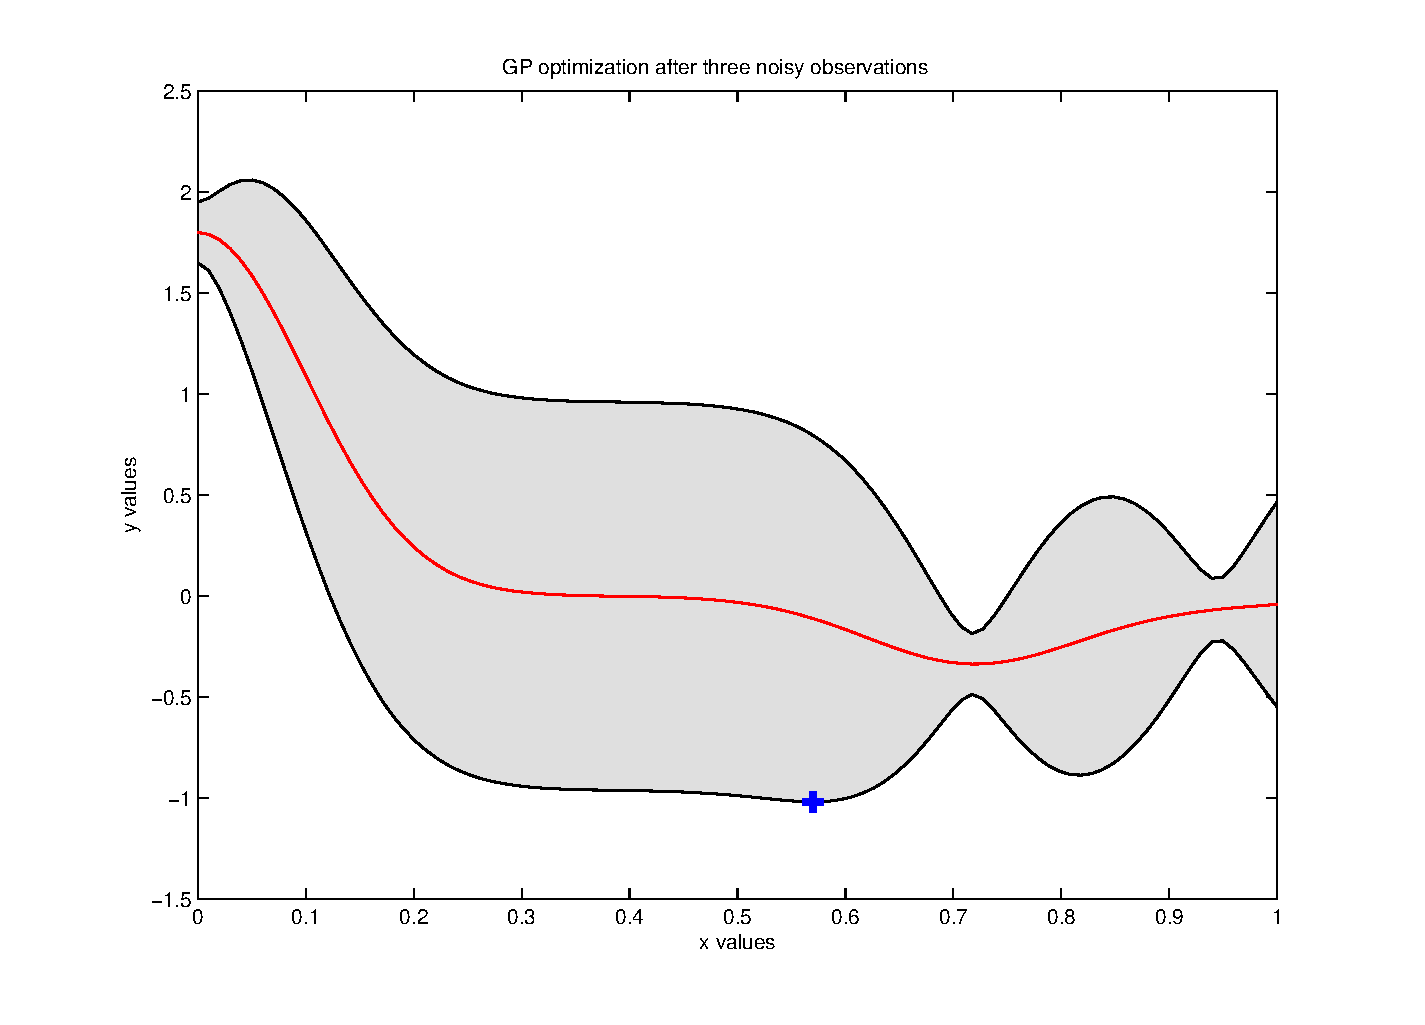
\includegraphics[scale=0.40]{test_gpucb1.eps}			
\caption{GPUCB optimization at time step 4}
\label{fig:gpucb1}
\end{figure}

\begin{figure}
\center
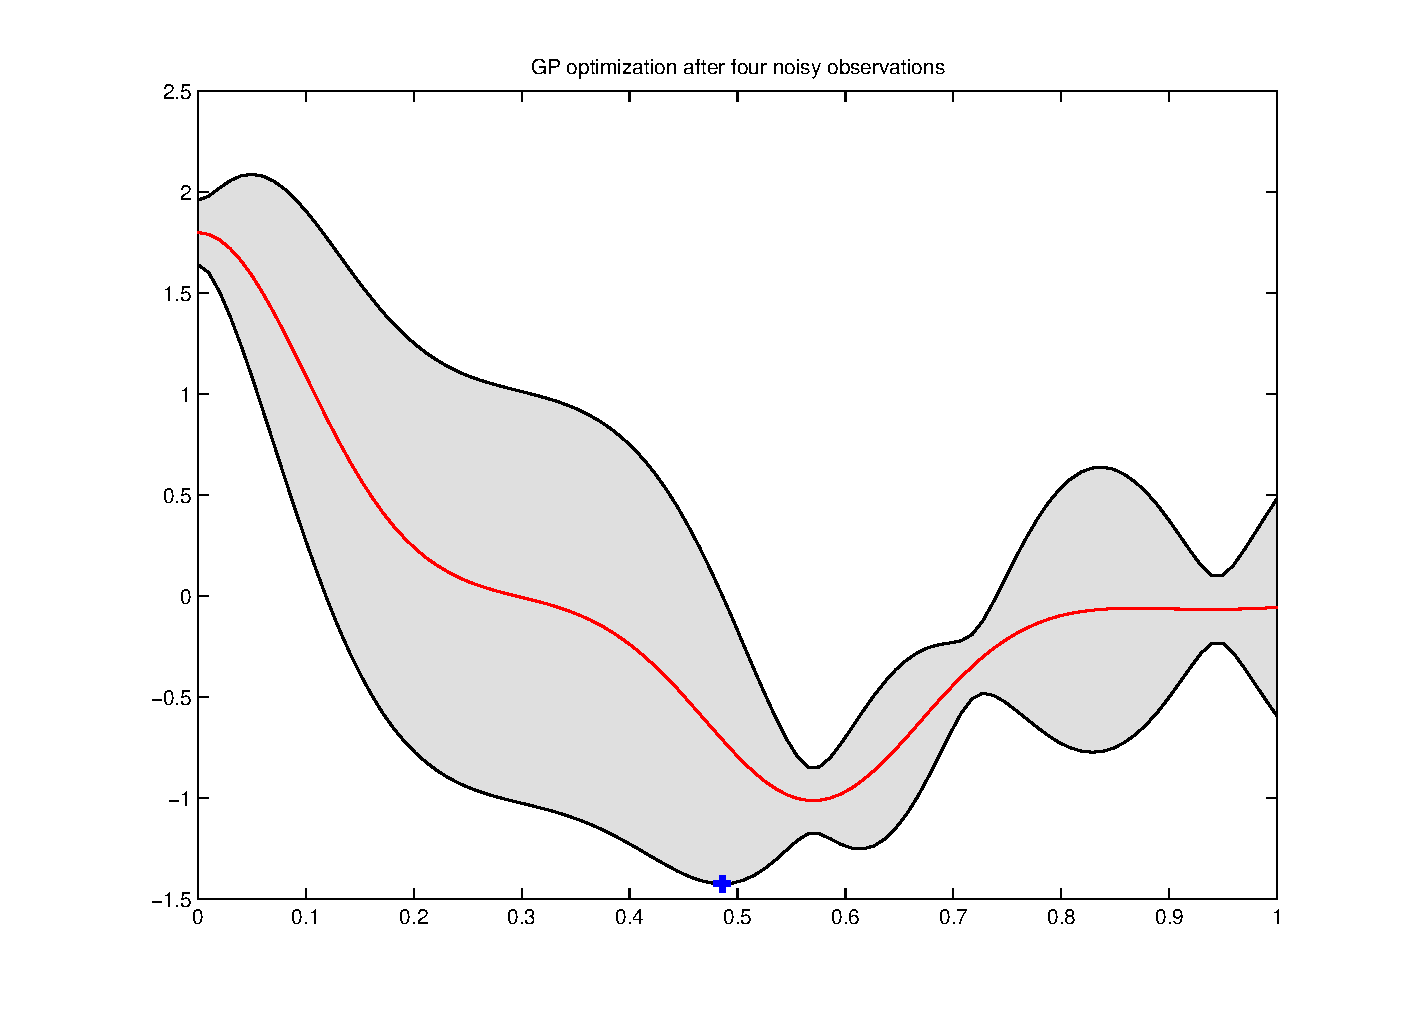
\includegraphics[scale=0.40]{test_gpucb2.eps}			
\caption{GPUCB optimization at time step 5}
\label{fig:gpucb2}
\end{figure}

The cumulative regret shown in Figure \ref{fig:cumregret} is averaged over 50 trials. For the $\beta_{t}$ value, Theorem 2 has been used, but it has been scaled down by 20. That is:

\begin{equation}
\beta_{t} = \frac{2 \log(t^{2}2 \pi^{2}/(3\delta)) + 2d\log(t^{2}dbr\sqrt{\log(4da/\delta)})}{20} \label{Thm2KrauseBeta}
\end{equation}

where $a = 1, b = 1, d = 1, r = 1$ and $\delta = 0.1$. 

\begin{figure}[h!t]
\center
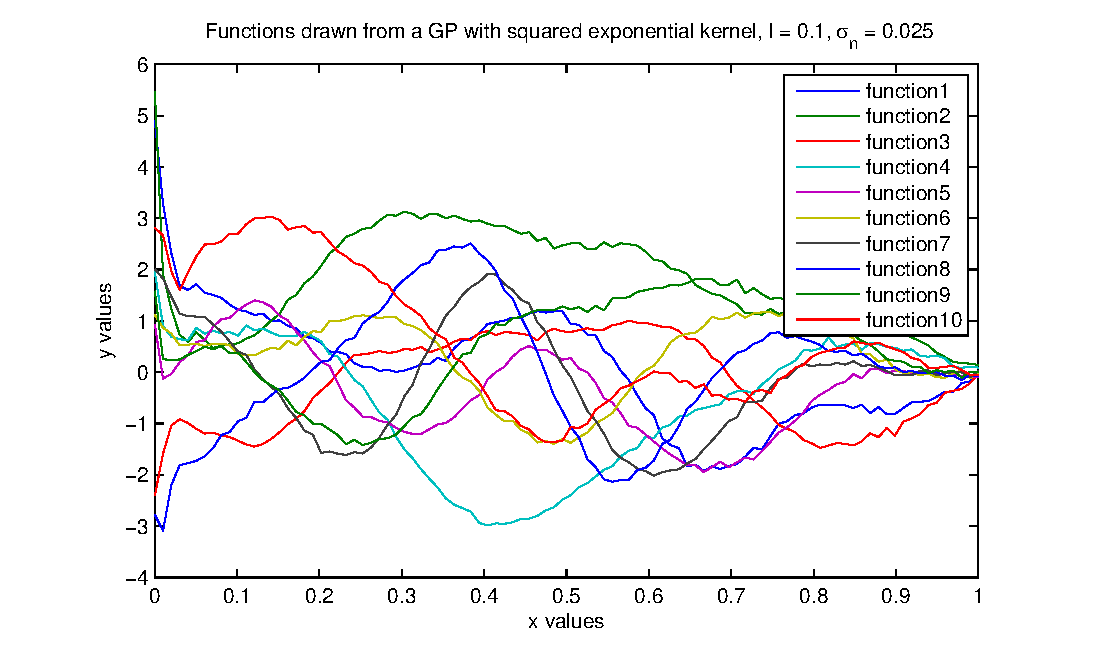
\includegraphics[scale=0.50]{functions.eps}			
\caption{Functions sampled from a Gaussian Process}
\label{fig:func}
\end{figure}

\begin{figure}[h!t]
\center
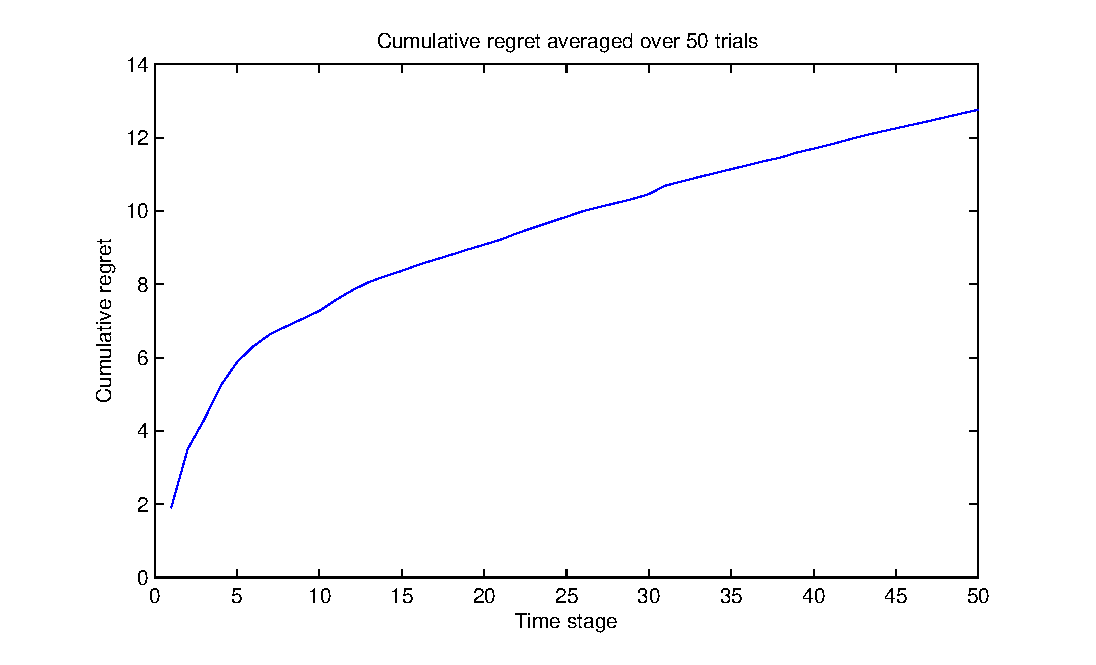
\includegraphics[scale=0.50]{test_cumregret.eps}			
\caption{Cumulative regret averaged over 50 trials}
\label{fig:cumregret}
\end{figure}

The shape of the cumulative regret growth agrees with the theoretical $\mathcal{O}(T^{1/2})$ growth. 

\section{Related Work}

Gaussian Processes are increasingly applied in control, where they are used to learn the unknown system dynamics. In \cite{Blimp} the authors propose a hybrid-GP approach combined with reinforcement learning to control an autonomous blimp. 
This approach closely parallels that of ours, the main differences lie in the use of the scalar cost function and the CGP-UCB framework, as will be detailed in the next sections. Their framework requires them to model the dynamics itself with a GP, and this is computationally very prohibitive as the number of dimensions increase. In \cite{PILCO,Deisenroth} the authors first learn the dynamics with GP. In the second step policies for a parameterized controller are learnt by propagating through the GP model. This method involves necessarily long offline calculations and many repeated trials. The method proposed in this paper aims to learn at every stage by incorporating feedback, and learns \emph{only} the stage cost, as a function of input and context, as opposed to the whole dynamics.

Gaussian process optimization literature proposes several heuristics such as Expected Improvement \cite{Jones01ataxonomy} and Most Probable Improvement \cite{Lizotte07automaticgait} for trading off exploration and exploitation. The first method with provable sublinear regret was proposed in \cite{Krause1}. The results of \cite{Krause1} were extended to the contextual setting in \cite{Krause2}, which is applied to dynamical systems in this thesis.

\chapter{Trajectory Tracking} \label{Chapter1}
% Open problems
% introduce Pontryagin equations and talk about perturbation analysis

%%%%%%%%%%%%%%%%%
% PUT AS PLOT
% learning result on pendulum balance up

\section{Iterative Learning Control} \label{ILC}
% start with Arimoto 1984

Iterative Learning Control (ILC) was first introduced in \cite{Arimoto} as a reference tracking methodology that learns to track the trajectory through iterations of an identically repeated trial.
See \cite{Survey} for a detailed survey of the subject. Here we go briefly over a particular optimization-based ILC method that appeared recently in \cite{ILC_Angela}.

The method consists of two separate steps: \emph{disturbance estimation} and \emph{input update} steps. For disturbance estimation through iterations, a time-varying Kalman filter is designed. The estimated disturbance will then be fed in as input to the optimization step, where the control objective is formulated as a (constrained) convex optimization problem. 

\subsection{Lifted Domain Representation}\label{LiftedDomain}

It is assumed that a nominal model of the dynamical systems is available from the start. The nominal model dynamics

\begin{align}
\dot{\state}(t) &= f(\state(t), \sysInput(t), t) \\
\observations(t)       &= g(\state(t), t)
\end{align}

where $\state(t)$ is the state vector, and $\observations(t)$ the observation at time $t$, is first linearized around an a priori determined output trajectory $\observations^{*}(t)$:

\begin{align}
\dot{\tilde{\state}}(t) &= A(t)\tilde{\state}(t) + B(t)\tilde{\sysInput}(t) \label{linX} \\
\tilde{\observations}(t) &= C(t)\tilde{\state}(t) \label{linY}
\end{align}

where 

\begin{align}
A(t) &= \frac{\partial{f(\state(t), \sysInput(t), t)}}{\partial{\state}} \\
B(t) &= \frac{\partial{f(\state(t), \sysInput(t), t)}}{\partial{u}} \\
C(t) &= \frac{\partial{g(\state(t), t)}}{\partial{\state}}
\end{align}

are the Jacobians of $f$ and $g$ with respect to $\state$ and $\sysInput$. Here the tilde signs correspond to deviations from the reference trajectory and input:

\begin{align}
\tilde{\sysInput}(t) &= \sysInput(t) - \sysInput^{*}(t) \\
\tilde{\state}(t) &= \state(t) - \state^{*}(t) \\
\tilde{\observations}(t) &= \observations(t) - \observations^{*}(t)
\end{align}

See Appendix \ref{app:trjgen} for details on how to generate the reference input signal $\sysInput^{*}(t)$ given output signal $\observations^{*}(t)$.

For a fixed discretization $h$, assuming a constant input signal between times $t$, and $t+h$ (also known as \emph{zero-order hold} in the control community), we can discretize the equations (\ref{linX}) and (\ref{linY}) as follows:

\begin{align}
\tilde{\state}(k+1) &= A_{D}(k)\tilde{\state}(k) + B_{D}(k)\tilde{\sysInput}(k) \label{discX} \\
\tilde{\observations}(k+1) &= C_{D}(k+1)\tilde{\state}(k+1) \label{discY}
\end{align}

These discretized matrices are 

\begin{align}
A_{D}(k) &= e^{A(k)h} \label{discrA} \\
B_{D}(k) &= A^{-1}(k)(A_{D}(k) - I)B(k) \label{discrB} \\
C_{D}(k) &= C(k)
\end{align}

(\ref{discrA}) and (\ref{discrB}) can be efficiently implemented by noting:

\begin{equation*}
\exp^{h \left(
\begin{BMAT}(rc){c:c}{c:c}
A(k) & B(k) \\
0 & 0
\end{BMAT} 
\right)}
= 
\left(
\begin{BMAT}(rc){c:c}{c:c}
A_{D}(k) & B_{D}(k) \\
0 & I
\end{BMAT} 
\right)
\end{equation*}

After discretization, the vectors $\tilde{\sysInput}$, $\tilde{\state}$, and $\tilde{\observations}$ can be stacked together to form the lifted vector representation of the dynamics:

\begin{align}
\state &= F\sysInput + d^{0} \label{liftedX} \\
\observations &= G\state \label{liftedY}
\end{align}

Here the lifted matrix is a block matrix of the following form:

\begin{equation}
F = 
\left(
\begin{array}{ccc}
F_{(1,1)} & \ldots & F_{(1,N)} \\
\vdots & \ddots & \vdots \\
F_{(N,1)} & \ldots & F_{(N,N)} 
\end{array} \right)
\end{equation}

where each entry is as follows:

\begin{equation}
F_{(i,j)} = 
\left\{
\begin{array}{cccc}
A_{D}(i-1) & \dotsi & A_{D}(j)B_{D}(j-1) & \text{if } j < i,\\
B_{D}(j-1) & & & \text{if } j = i,\\
0 & & & \text{if } j > i.
\end{array} 
\right\}.
\end{equation}

The matrix $G$ is only block diagonal, with entries consisting of $C_{D}$ matrix stacked diagonally.
The vector $d^{0}$ is the \emph{free response} of the system to the initial deviation $\tilde{\state}(0)$. The initial deviation from the reference trajectory $\state^{*}(t)$ is the only disturbance in this model. The static linear mapping (\ref{liftedX}) - (\ref{liftedY}) is a useful formulation for ILC, since each iteration can be described succinctly in this way. Extending it to many iterations, indexed by $l$, and more general disturbances (due to unmodeled dynamics, parameter mismatch, etc.) we get:

\begin{align}
\state_{l} &= F\sysInput_{l} + d_{l} + N_{\xi}\xi_{l} \label{liftedXiter} \\
\observations_{l} &= G\state_{l} + N_{\nu}\nu_{l} \label{liftedYiter} \\
d_{l} &= d_{l-1}	+ \omega_{l-1} \label{dEvolution}	
\end{align}

\subsection{Disturbance estimation}
\label{ILC_Kalman}

The process noise signal $\xi$ in (\ref{liftedXiter}) and the measurement noise signal $\nu$ in (\ref{liftedYiter}) are both zero-mean Gaussian white noise with unit variance, $\xi, \nu \sim \mathcal{N}(0,1)$.
(\ref{dEvolution}) is a model describing the evolution of the disturbance. This model is necessary in order to approach the problem from the standard Kalman filter perspective. The dynamics of the disturbance is then as follows:

\begin{equation}
\begin{aligned}
d_{l} &= d_{l-1}	+ \omega_{l-1} \\
\observations_{l} &= Gd_{l} + GF\sysInput_{l} + \mu_{l} \label{DisturbanceDynamics}
\end{aligned}
\end{equation}

Here $\omega_{l} \sim \mathcal{N}(0, M_{l})$ is just another zero-mean Gaussian white noise signal, modelling a slight variation in $d$. For a critique of this approach, see section \ref{critique}. The output noise in (\ref{DisturbanceDynamics}) is the stacking of process and noise signals, i.e. $\mu = G N_{\xi}\xi_{l} + N_{\nu}\nu_{l}$, $\mu_{l} \sim \mathcal{N}(0, \Omega_{l})$. 

% Kalman filter update equations
% refer to article for tuning covariance matrices for faster/better range of convergence.
Kalman filter update equations for the dynamics given in (\ref{DisturbanceDynamics}) are as follows:

\begin{align}
S_{l} &= P_{l-1} + \Omega_{l-1} \\
K_{l} &= S_{l}G^{\mathrm{T}}(GS_{l}G^{\mathrm{T}} + M_{l})^{-1} \\
P_{l} &= (I - K_{l}G)S_{l}
\label{Kalman}
\end{align}

Here $P_{l} = E[(d_{l} - \hat{d}_{l})(d_{l} - \hat{d}_{l})^{\mathrm{T}}]$ is the covariance of the disturbance $d_{l}$. If $P_{0}$ and $\hat{d}_{0}$ are provided as initial values, the Kalman filter will update the Kalman gain $K_{l}$ at each iteration and estimate $d_{l}$ as:

\begin{equation}
\hat{d}_{l} = \hat{d}_{l-1} + K_{l}(\observations_{l} - G\hat{d}_{l-1} - GF\sysInput_{l})
\end{equation}

The performance of the estimation is dependent on the design parameters, the covariance matrices $\Omega_{l}, M_{l}$ and initial values $P_{0}$ and $\hat{d}_{0}$. More information on the tuning of such parameters can be found in \cite{ILC_Angela}. 

\subsection{Input Update}

In the input update step, the objective is to find the next control input difference $\sysInput_{l+1}$ which will compensate for the estimated disturbance in some optimal sense. Then the total applied input in the next iteration will be $\sysInput(t) = \sysInput^{*}(t) + \sysInput_{l+1}(t)$. Here, the expected value of the deviation from the reference trajectory 

\begin{equation}
E[\state_{l+1}|\observations_{1}, \ldots, \observations_{l}] = F\sysInput_{l+1} + \hat{d}_{l}
\end{equation}

is to be minimized, i.e. the following optimization problem is solved at each step:

\begin{equation}
\begin{aligned}
\sysInput_{l+1} &= \argmin_{\sysInput} ||F\sysInput + \hat{d}_{l}||_{2} \\ 
& \text{subject to } L\sysInput \leq q
\end{aligned}
\end{equation}

Refer to the article \cite{ILC_Angela} for additional tuning such as derivative norm penalties, optimization under different norms, and scaling for better and smoother performance. Constraint $L, q$ formulation is not given here but constraints can be transformed around the reference trajectory, discretized and formed into the \emph{lifted vector representation} along with the process detailed in \ref{LiftedDomain}.

\subsection{Analysis of the method}\label{critique}

% % % % % % % % % % % % % % % % %
% critique: the Kalman filter approach is wrong
The method works very well in cases where the nominal model of the dynamical system under consideration is not far off from the real dynamics of the system. In this case the method will converge in very few iterations. The performance of the method is presented in the results section \ref{Results1} in two example problems. However the proposed standard Kalman filter approach is an \emph{ad hoc} solution to the estimation problem and will not be effective in estimating large disturbances. To see this, let us consider a more complete description of the system, denoted as \emph{real}:

\begin{align}
\dot{\state}(t) &= f_{real}(\state(t), \sysInput(t), t) \\
\end{align}

This system can also be linearized around a reference trajectory $\state^{*}(t)$, discretized, and then \emph{lifted} to form the lifted-vector representation. Assuming, for simplification, that the states themselves are fully observed, i.e. $\observations(t) = \state(t)$, and stacking process and measurement noises in $\mu$ we obtain:

\begin{align}
\state_{l} &= F_{nom}\sysInput_{l} + d_{l} + \mu_{l} \label{liftedXiterNom} \\
d_{l} &:= \Delta F \sysInput_{l} = (F_{real}-F_{nom})\sysInput_{l} \label{dEvolutionReal}	
\end{align}

Here $d_{l}$ in (\ref{dEvolutionReal}) cannot be estimated by a Kalman filter because the matrix $\Delta F$ is not known. Instead the matrix $\Delta F$ should be estimated from the previous iteration results:

\begin{align}
\mathbf{v}_{l} &:= \state_{l} - F_{nom}\sysInput_{l} \\
\mathbf{v}_{l} &= \Delta F \sysInput_{l} + \mu_{l}
\end{align}

The matrix should hence be estimated from noisy outputs $\mathbf{v}_{l}$ and inputs, where $\sysInput_{l}$, $l = 1, \ldots, N$, and $N$ the total number of iterations up to the estimation. The problem falls under the category of \emph{exploration-exploitation} because simultaneously while estimation of the matrix difference $\Delta F$ is critical, the real objective is to the drive the deviation signal $\state_{l}$ to zero.

% mention perhaps the special sparse structure of deltaF

Another important problem with the method is the linearization around a reference trajectory. This linearization is only accurate for small disturbances around the trajectory, and will prevent the method from converging under wider model mismatches. An important research topic would be to characterize under which conditions the method converges and consider whether it is possible to still achieve learning feed-forward control signals \emph{without} linearizing around a trajectory.

% on stability and safety
% limitations
As a final point, note that stability is also not guaranteed with this method. In fact, it is assumed that the motion of the system stays close to the reference trajectory during the learning process and has to be enforced otherwise by stopping and restarting the whole iteration.

% % % % % % % % % % % % % % % % % 
These considerations all lead us away from ILC and into machine learning methodologies adapted to control, one of which is the learning algorithm CGP-UCB introduced in \ref{ContextBandit}.

%\section{Model Predictive Control}
% present the main idea behind MPC.
% approximating the value function
% learning result on 2-d robot kinematics with ILC as comparison

\section{Problem Setting and Methodology} 
\label{methodology}
%%%%%%%%%%%%%%%%%
% Include the derivation of example delta J

\subsection{Optimal Control}
% references needed!!!
Consider the following system dynamics: 

\begin{equation}
\dot{\state}_t = f(\state_t,\sysInput_t), \quad  t \geq 0,
\label{eq:readDynamics}
\end{equation}

where $\state_t \in \mathbb{R}^n$ denotes the state of the system at time $t$ and $\sysInput_t \in \mathbb{R}^m$ denotes the control input.  

In continuous time optimal control, the control objective at time $\tau, \, 0 \leq \tau \leq T$ can be given as follows:

% % % % Add the terminal cost
\begin{equation}
\begin{aligned}
\sysInput^{*}(t) &= \argmin_{\sysInput \in D} J(\sysInput) \quad \text{subject to} \\
\dot{\state}_t &= f(\state_t,\sysInput_t), \quad  t \geq \tau
\end{aligned}
\label{optimalControl}
\end{equation}

where $J(\sysInput)$ is the cost functional defined by:

\begin{equation}
J(\sysInput) = \int\limits_{t = \tau}^{T} (\state(t) - \state^{*}(t))^{\mathrm{T}}Q(t)(\state(t) - \state^{*}(t)) + \sysInput(t)^{\mathrm{T}}R(t)\sysInput(t) \label{costFunctional}
\end{equation}

$D$ denotes the constraints imposed on the dynamics. $Q$ and $R$ are matrices penalizing the deviations from the defined trajectory and the control input, respectively. They are generally taken to be diagonal with constant nonnegative entries. Zero diagonal entries correspond to states that are not actively tracked. In the limit as $T$ goes to infinity, the optimization in (\ref{costFunctional}) becomes the infinite-horizon optimal control problem. In this case $Q(t)$ and $R(t)$ must be decaying sufficiently fast to make $J(\sysInput)$ finite. 

% reference needed
A necessary condition for a control signal $\sysInput(t)$ to be an optimal solution of (\ref{optimalControl}) is that it should satisfy \emph{Pontryagin's minimum principle}. A necessary and sufficient condition is that $\sysInput(t)$ should be a solution of the \emph{Hamilton-Jacobi-Bellman} (HJB) partial differential equation \cite{Bertsekas:DP01}.

Assuming zero-order hold and an Euler discretization of (\ref{costFunctional}), we get the following:

\begin{equation}
J(\sysInput) = \sum\limits_{i = \tau_{h}}^{N} (\state_{i} - \state_{i}^{*})^{\mathrm{T}}Q(\state_{i} - \state_{i}^{*}) + \sysInput_{i}^{\mathrm{T}}R\sysInput_{i} \label{costDiscrete}
\end{equation}

where $\tau_{h} \geq \tau/h$ is the next time stage under the discretization $h = T/N$. From now on we will consider $R$ to be zero and only concentrate on the costs caused by the trajectory deviations. Rewriting (\ref{costDiscrete}) in a more convenient form:

\begin{equation}
J(\sysInput) = \sum\limits_{i = \tau_{h}}^{N} ||\state_{i} - \state_{i}^{*}||_{Q}^{2} \label{costNormed}
\end{equation}

A solution $\sysInput(t)$ of this discrete formulation should satisfy Bellman's equations, the discrete form of the HJB equations. In the finite horizon case, this solution can be calculated recursively using Dynamic Programming, and in the infinite-horizon case, using Policy Iteration or Value Iteration algorithms. See \cite{Bertsekas:DP01} for details. These algorithms all suffer from the \emph{curse of dimensionality} and they are computationally very inefficient in high-dimensional state spaces. This is because they have to consider \emph{non-greedy} policies to calculate an optimal solution. Non-greedy policies can be avoided in cases where the desired trajectory $\state^{*}(t)$ is always \emph{feasible}. More precisely, we have the following: \\

% which assumptions can we remove/relax ?
\begin{proposition}[Dissociation of stage costs]
The finite horizon optimal control problem with the cost given in (\ref{costNormed}) under zero-noise assumption\footnote{Here we include any unknown dynamics as a disturbance that contributes to the noise signal.} reduces to sequential greedy stage-cost minimization given that the trajectory $\state^{*}(t)$ is \emph{feasible} throughout, i.e. $\forall t \ \ \exists \sysInput \ \ s.t. \ \ \state^{*}(t+h) = f_{h}(\state(t), \sysInput(t), t)$.
\label{Prop:1}
\end{proposition}

\begin{proof}
The proof is trivial. First we note that the finite horizon optimal control problem under the zero-noise assumption can be posed as a non-stochastic \emph{shortest path problem} which can be solved iteratively instead of recursively. At time stage $t \ $:

\begin{equation*}
J^{*}_{t}(\sysInput_{t:N}) = \min_{u_{t}}(J_{t}(u_{t}) + J^{*}_{t+1}(\mathbf{U}_{t+1:N}))
\end{equation*}

where $\sysInput_{t:N} = (u_{t}, \ldots, u_{N})$, future inputs stacked together. Since each $J_{t}(u_{t}) = 0$ due to the feasibility assumption for all $t$, the optimal cost to go $J^{*}_{t}(\sysInput_{1:N}) = 0$. But we can always achieve this cost by minimizing the stage cost $J_{t}(\sysInput_{t}) = 0$ greedily.

\end{proof}

Here $f_{h}$ is the discretized version of (\ref{eq:readDynamics}):

\begin{equation}
\state_{t+h} = f_{h}(\state(t), \sysInput(t), t) = \state_{t} + \int_{t}^{t+h}f(\state_{t'},\sysInput_t)dt' \label{eq:realDynamics_discrete}
\end{equation}

Zero-noise including the perfectly known model assumption in Proposition \ref{Prop:1} is obviously too stringent. Here we conjecture that this assumption can be somewhat relaxed and the proposition will still hold, at least in a probabilistic sense. If it is possible to put a probabilistic bound on the noise and the deviation due to model mismatch, then we can plan feasible (with high probability) trajectories on the state space with these bounds in mind, and still expect to achieve good performance with a greedy optimization. More precisely, in terms of \emph{stability} theory, we would like to stabilize the system dynamics around the trajectory.

% % % % update on this
\subsection{Stability}
\label{stability}
If the tracked states deviate by a large margin from the desired trajectory during an initial run, the next state to go to, $\state^{*}_{t+h}$ will have to be recalculated instead to avoid violating input constraints. Given a trajectory of horizon of size $T$ and a method $H(\state(t), \state^{*}(t+h), \ldots, \state^{*}(t+Th))$ for calculating a converging trajectory over the horizon:
\begin{equation}
\state^{*}_{new}(t+h) = H(\state(t), \state^{*}(t+h), \ldots, \state^{*}(t+Th)) \label{converging_trj} \\
\end{equation}
This method $H$ can be used to speed up the convergence of the proposed method over time. 
Of course since the disturbance dynamics is not known exactly, such a method can only generate \emph{feasible} converging trajectories probabilistically. Over time however, the disturbance dynamics will be more or less known around the traversed state-space points, and converging trajectories will be asymptotically stable with high probability (w.h.p.). We have the following:

% first attempt at proposition
% add CGP-UCB assumptions: that the cost function is a GP with known parameters, or known RKHS bound
\begin{proposition}[Stability]
Assume that we have a method $H$ that can compute converging trajectories w.h.p. $p \leq 1 - \delta_{1}$. If this method incurs over time $T$ cumulative regret on the order $\mathcal{O}(T^{\alpha})$, $\alpha < 1$ w.h.p. $p \leq 1 - \delta_{2}$, then for the inputs calculated using CGP-UCB, the dynamics is asymptotically stable w.h.p. $p = 1 - \delta, \, \delta \geq \delta_{1} + \delta_{2}$.
\label{Prop:1}
\end{proposition}

\begin{proof}
Since regret at time stage $t$ is $r_{t} = J(\sysInput_{t}) - J(\sysInput^{*})$, where $\sysInput^{*} = \operatorname*{arg\,min}_{u \in U(t)} \|\state_{t+h} - \state^{*}_{t+h}\|_{Q}^{2}$, the cumulative regret at time stage $T$:

\begin{equation}
R_{T} = \sum_{t=1}^{T}r_{t} = \sum_{t=1}^{T}J(\sysInput_{t}) - J(\sysInput^{*}) \label{cumRegret}
\end{equation}

$R_{T}$ is of order $\mathcal{O}(T^{1/2})$ w.h.p $1-\delta_{1}$, hence assuming that the method $H$ incurs regret of order $\mathcal{O}(T^{\alpha})$, $\alpha < 1$ w.h.p $1-\delta_{2}$, the regret for $H$ being defined by:

\begin{equation}
r_{t}^{\mathrm{H}} = J(\sysInput^{*}|\state^{*}_{t+h}) - J(\sysInput^{*}|\state^{\mathrm{H}}_{t+h})
\end{equation}

where $\state_{t+h}^{\mathrm{H}}$ is any feasible next state such that $J(\sysInput^{*}|\state_{t+h}^{\mathrm{H}}) = 0$, then the total cost to go

\begin{align}
\sum_{t=1}^{T}J(\sysInput_{t}) &= \sum_{t=1}^{T}\Delta\state^{\mathrm{T}}Q\Delta\state = \mathcal{O}(T^{\beta}), \\ & \text{w.h.p. } 1 - \delta, \quad \delta \geq \delta_{1} + \delta_{2} \\
\beta &= \max(1/2, \alpha) < 1
\end{align}

This implies that $\lim_{T \to \infty} \Delta\state^{\mathrm{T}}Q\Delta\state = 0$ w.h.p. For positive definite $Q \ $, $\lim_{T \to \infty} \Delta\state = 0$ w.h.p.

\end{proof}

Here method $H$ acts as a magnet around the trajectory, making sure that the trajectories do not deviate over time $T$ by more than $\mathcal{O}(T^{\alpha})$. $H$ can be constructed by noting \eqref{function bound}: converging trajectories should be chosen such that the uncertainty is smallest. This task gets easier as the variance $\sigma^{2}$ decreases over time.

%converging trajectories
\subsection{Stage Cost Minimization}
\label{StageCostMin}

The control objective at time $t$ is to track the desired state at the next time step $\state^{*}_{t+h}$, that is minimizing the following stage cost:

\begin{equation}
J_{t} := \|\state_{t+h} - \state^{*}_{t+h}\|_{Q}^{2}. \label{eq:stagecost}
\end{equation}

Furthermore, assume a nominal model of the system given in (\ref{eq:readDynamics}) is known and given by

\begin{equation}
\dot{\state}_t = f_{\mathrm{nom}}(\state_t,\sysInput_t) \label{nominal_model} \\.
\end{equation}

Note that the above nominal model is typically derived from first principles. This nominal model is only an approximation of (\ref{eq:readDynamics}) and the unmodelled dynamics can be seen as repeating disturbances that can be learned using the CGP-UCB framework introduced in \ref{ContextBandit}.

Tracking the global minimum of the stage cost (\ref{eq:stagecost}) results in solving the following optimization problem at each time step:

\begin{equation}
\begin{aligned}
\sysInput_{t} &= \operatorname*{arg\,min}_{u \in U(t)}\|\state_{t+h} - \state^{*}_{t+h}\|_{Q}^{2} \\
\state_{t+h} &= \state_{t} + \int_{t}^{t+h}f(\state_{t'},\sysInput_t)dt'
\end{aligned}
\label{stageCostOptim}
\end{equation}

where $U(t) \subset \mathbb{R}^m$ is the feasible input space at time step $t$, assuming zero-order hold. But system dynamics $f$ in (\ref{stageCostOptim}) is not known. However, since we have a nominal model, we can learn $f$ indirectly by just learning the difference in cost predicted by the nominal model and the actual cost:

\begin{equation}
\|\state_{t+h} - \state^{*}_{t+h}\|_{Q}^{2} - \|\hat{\state}_{t+h} - \state^{*}_{t+h}\|_{Q}^{2} \label{eq:deltaJ}
\end{equation}

where 
\begin{equation}
\hat{\state}_{t+h} = \state_{t} + \int_{t}^{t+h}f_{\mathrm{nom}}(\state_{t'},\sysInput_t)dt' \label{eq:nominal_discrete}
\end{equation}

is the predicted state using the nominal model.

The above cost given in (\ref{eq:deltaJ}) can also be rewritten to show explicit dependence on context and repeating disturbances:

\begin{align}
\Delta J_{t} &: (\state_t, \state^{*}_{t+h}; \sysInput_t) \mapsto \Delta F^{\mathrm{T}} Q \Delta F + 2(\hat{\state}_{t+h} - \state^{*}_{t+h})^{\mathrm{T}} Q \Delta F \label{delta_cost} \\
\Delta F &:= \int_{t}^{t+h}f(\state_{t'},\sysInput_t)dt' - f_{\mathrm{nom}}(\state_{t'},\sysInput_t)dt' \label{delta_f} 
\end{align}

where $\state_t \times \state^{*}_{t+h} \in C$, the context space, and $\sysInput_t \in U(t)$. This whole process, in terms of the CGP-UCB optimization, translates into adding the nominal model predicted cost $\|\hat{\state}_{t+h} - \state^{\mathrm{*}}_{t+h}\|_{Q}^{2}$, a known function of $\sysInput$, as a prior mean in (\ref{ucb}):

\begin{equation}
\sysInput_{t} = \operatorname*{arg\,min}_{u \in U(t)} \left\lbrace  \|\hat{\state}_{t+h} - \state^{*}_{t+h}\|_{Q}^{2} \right. 		+ \mu(\sysInput;\context) - \beta_t^{1/2}\sigma(\sysInput;\context) \rbrace \label{boostedUCB}
\end{equation}

This known component of the mean function thus does not have to be estimated during hyperparameter estimation. We believe the performance of the proposed method is very sensitive to changes in the mean function parameters, and hence by adding the nominal cost, we are ensuring more robustness with respect to hyperparameter estimation. 

\subsection{Examples}
\label{examples}
% here examples from the quadrocopter
As an example consider the quadrocopter model. A two-dimensional model of the quadrocopter dynamics derived from first principles can be given as follows \cite{ILC_Angela}:

\begin{equation}
\begin{aligned}
\ddot{y} &= -f_{\mathrm{coll}} \sin\phi \\
\ddot{z} &=  f_{\mathrm{coll}}\cos\phi - g \\
\dot{\phi} &= \omega_{x}
\end{aligned}
\label{quadrocopterDynamics}
\end{equation}

where state $\state = (y,\dot{y},z,\dot{z},\phi)$. The states $y, z$ are trajectories to be tracked, corresponding to the horizontal and vertical axes and the control input $\sysInput = (f_{\mathrm{coll}}, \omega_x)$, where $f_{\mathrm{coll}}$ is the collective thrust and $\omega_x$ is rate of change of the angle of attack with respect to the x-axis. Constraints are given in Appendix \ref{app:trjgen}, see Table \ref{table_parameters} and (\ref{thrust_constraints}) -- (\ref{angular_vel_constraints}). 

Unmodeled dynamics in quadrocopters could be due to parameter mismatch (e.g. gravity difference) or a more general repeating disturbance (e.g. a fan).

\textit{Example 1}. As an analytical example consider a quadrocopter operating in another planet, whose nominal model represents the quadrocopter flying in Earth. Gravity difference $\Delta g$ using Euler discretization (with time discretization $h$) and $Q$ as the identity matrix, causes the following cost difference at each time stage:

\begin{equation}
\Delta J(\state,\state^{*};\sysInput) = h^{2}(\Delta g)^{2} - 2h^{2}g\Delta g + 2h\Delta g(s_{4}-s^{*}_{4}) + 2h^{2}\Delta g u_{1} \cos s_{5} \label{example1General} 
\end{equation}

In Mars, the huge gravity difference ($g_{mars} = 3.75, g_{earth} = 9.81$), and $h = 0.02$ causes the following cost difference:

\begin{equation*}
-0.0329 + 0.2424(s_{4} - s^{*}_{4}) + 0.0048u_{1}\cos s_{5} \label{exampleMars} 
\end{equation*}

where $s_{4}$ is the $\dot{z}(t)$, $s_{5}$ is $\dot{\phi}(t)$, $s^{*}_{4}$ is the $\dot{z}(t+h)$ along the trajectory and $u_{1}$ is the collective thrust $f_{\mathrm{coll}}$. We effectively learn this function $\Delta J(\state, \state^{*}; \sysInput): \mathbb{R}^{3} \times \mathbb{R} \mapsto \mathbb{R}$, as we do online CGP-UCB optimization along the trajectory.

\textit{Example 2}. As another example consider the effect of constant wind on the quadrocopter operation. Assuming the wind, coming at an angle of $\theta$ from the horizontal axis, exerts a pressure $P_{wind}$ on the quadrocopter with area $A$, the dynamics (\ref{quadrocopterDynamics}) is modified as follows: 

\begin{align}
\ddot{y} &= -f_{\mathrm{coll}} \sin\phi \label{yddot} + P_{wind} A sin(\theta + \phi) cos \theta \\
\ddot{z} &=  f_{\mathrm{coll}} \cos\phi - g \label{zddot} + P_{wind} A sin(\theta + \phi) sin \theta \\
\dot{\phi} &= \omega_{x} \label{phidot}
\end{align}

The cost difference (again using Euler discretization and identity matrix for $Q$) is shown below:

\begin{equation}
\begin{aligned}
& \Delta J(\state,\state^{*};\sysInput) = h^{2}P_{wind}^{2}A^{2} \sin^{2}(s_{5} + \theta)  \\
& \hspace*{2em} + 2hP_{wind}A\sin(s_{5} + \theta)((s_{2} - s^{*}_{2})\cos\theta + (s_{4} - s^{*}_{4})\sin\theta)  \\
& \hspace*{2em} - 2h^{2}P_{wind}Au_{1}\sin(s_{5} - \theta)\sin(s_{5} + \theta) \\
& \hspace*{2em} - 2h^{2}P_{wind}Ag\sin\theta\sin(s_{5} + \theta) 
\end{aligned}
\label{example2General}
\end{equation}

Assuming a perfectly horizontal wind, i.e. $\theta = 0$, cost difference is simplified:

\begin{align}
\Delta J(\state,\state^{\mathrm{*}};\sysInput) = (h^{2}P_{wind}^{2}A^{2} - 2h^{2}P_{wind}A\ u_{1}) \sin^{2} s_{5} + 2hP_{wind}A(s_{2} - s^{*}_{2})\sin s_{5} \label{QuadTheta0}
\end{align}
%

\subsubsection*{Derivation}
%%% Here put the derivation of the 2nd example and tie in with the 1st
(\ref{example2General}) can be derived using the stage cost difference equation (\ref{delta_cost}):

\begin{equation}
\begin{aligned}
\Delta J &= h^{2}\begin{pmatrix} 0 \\ P_{wind} A \sin(\theta + \phi) \cos \theta \\ 0 \\ P_{wind} A \sin(\theta + \phi) \sin \theta \\ 0
\end{pmatrix}^{\mathrm{T}}\begin{pmatrix} 0 \\ P_{wind} A \sin(\theta + \phi) \cos \theta \\ 0 \\ P_{wind} A \sin(\theta + \phi) \sin \theta \\ 0
\end{pmatrix} + \\
& \quad 2h(\hat{\state}_{t+h} - \state^{*}_{t+h})^{\mathrm{T}}\begin{pmatrix} 0 \\ P_{wind} A \sin(\theta + \phi) \cos \theta \\ 0 \\ P_{wind} A \sin(\theta + \phi) \sin \theta \\ 0
\end{pmatrix} \\
&= h^{2}P_{wind}^{2}A^{2}\sin^{2}(\theta + \phi) + 2h \begin{pmatrix} 0 \\ \Delta \dot{y} - hf_{\mathrm{coll}} \sin(\phi) \\ 0 \\ \Delta \dot{z} + hf_{\mathrm{coll}} \cos(\phi) - hg \\ 0 \end{pmatrix}^{\mathrm{T}}  \begin{pmatrix} 0 \\ P_{wind} A \sin(\theta + \phi) \cos \theta \\ 0 \\ P_{wind} A \sin(\theta + \phi) \sin \theta \\ 0 \end{pmatrix} \\
&= h^{2}P_{wind}^{2}A^{2}\sin^{2}(\theta + \phi) + 2hP_{wind}A \sin(\theta + \phi)(\Delta \dot{y} \cos\theta + \Delta \dot{z} \sin\theta) - \\ 
& \quad 2h^{2}P_{wind}Af_{\mathrm{coll}}\sin(\phi - \theta)\sin(\phi + \theta) - 2h^{2}P_{wind}Ag \sin(\theta + \phi) \sin\theta 
\end{aligned}
\label{derivationQuad}
\end{equation}

If $\theta = 0$ then all terms with $\sin \theta$ disappear, and we're left with (\ref{QuadTheta0}). If $\theta = \pi/2$ then (\ref{derivationQuad}) reduces to:

\begin{equation}
\Delta J = h^{2}P_{wind}^{2}A^{2}\cos^{2}\phi + 2hP_{wind}A\cos\phi(\Delta \dot{z} - hg) + 2h^{2}P_{wind}Af_{\mathrm{coll}}\cos^{2}\phi
\end{equation}

The acceleration is due to the wind force $P_{wind}A\cos\phi$. Replacing it with $\Delta g$,  we get 
(\ref{example1General}).

\section{Implementation}
\label{Implementation}
The process is summarized in Figure \ref{alg} in algorithmic form.

\begin{figure}[!hbp]
\begin{algorithmic}[1]
\REQUIRE $n$ example trajectories
\FOR{$i=1$ to $n$}
	\STATE $\Delta J(t) \leftarrow \|\state_{t+h} - \state^{\mathrm{*}}_{t+h}\|_{2}^{2} - \|\hat{\state}_{t+h} - \state^{\mathrm{*}}_{t+h}\|_{2}^{2} $
\ENDFOR
\STATE Search through models and fit hyperparameters
\LOOP[for a new trajectory]
	\FOR{$t=1$ to $T$}
		\STATE $\beta_{t} \leftarrow \beta(t,\delta, d, a, b, r)$
		\STATE $\context := (\state_t, \state^{*}_{t+h})$
		\STATE $\sysInput_{t} = \operatorname*{arg\,min}_{\sysInput \in U(t)} \left\lbrace  \|\hat{\state}_{t+h} - \state^{*}_{t+h}\|_{Q}^{2} \right. 		+ \mu(\sysInput;\context) - \beta_t^{1/2}\sigma(\sysInput;\context) \rbrace $
		\STATE $\state_{t+h} \leftarrow \state_{t} + \int_{t}^{t+h}f(\state,\sysInput_{t})dt'$
		\STATE $\Delta J(\sysInput_{t}) \leftarrow \|\state_{t+h} - \state^{*}_{t+h}\|_{Q}^{2} - \|\hat{\state}_{t+h} - \state^{*}_{t+h}\|_{Q}^{2} $
		\STATE Update GP (\ref{gpUpdate_mu}), (\ref{gpUpdate_sigma}) with $(\sysInput_{t}, \Delta J(\sysInput_{t}))$
	\ENDFOR
\ENDLOOP
\end{algorithmic}
\caption{CGP-UCB for trajectory tracking}
\label{alg}
\end{figure}

Before starting GP-optimization, we need to train the GP by estimating hyperparameters from gathered data. Hence the process starts in lines 1-3 with gathering the necessary evaluations for hyperparameter estimation from trial trajectory runs, i.e. contexts, actions, and cost differences. 

As mentioned in \ref{StageCostMin}, the current state and the desired next state constitute the contexts, $\ \state_t \times \state^{*}_{t+h} \in C$, and actions in these trial runs are the feedforward control inputs calculated using a nominal model. See Appendix \ref{app:math} for feedforward control signal generation of a differential flat system using the splines method. 

We then search for each kernel structure $\mathit{M}_i, i = 1, \ldots, m $ through the hyperparameter space for parameters maximizing the log likelihood of data. See Chapter \ref{Chapter2} for hyperparameter estimation.

In the main loop (lines 6-13), we start by updating $\beta(t)$, the constant that balances exploration-exploitation optimally. This constant plays a big role in the GP-UCB proofs \cite{Krause1} but its scale has not been optimized in the proofs. Hence we find that by dividing the theoretical beta-value given in Theorem 1 \cite{Krause1} by 5-20, we provide more aggression for optimization and increase overall performance. See equation (\ref{Thm2KrauseBeta}). Alternatively Reproducing Kernel Hilbert Space (RKHS) approach can also be used for sufficiently smooth cost functions. 
See (\ref{Thm3KrauseBeta}) in Chapter \ref{Chapter2} for details on this. 

The quantile-based distribution in line 9 is multi-modal in general. See section \ref{ControlAffine} for a QP formulation of this problem for control affine systems. In general the associated optimization will be non-convex. For non-convex optimization, we can use the \emph{DIRECT} (Dividing Rectangles) algorithm \cite{Jones:1993,Brochu}, which samples hierarchically through search space, or MATLAB's constrained global optimization routine \emph{fmincon}, among others.

If the system inputs are constrained to lie within a certain bounded set $U \subset \mathbb{R}^{n}$, then the optimization (\ref{boostedUCB}) should be constrained within that set. As a last step, GP is conditioned on the sampled control input and the cost difference incurred along the trajectory.  

\subsection{QP formulation for Control-Affine systems}
\label{ControlAffine}

Control-affine systems are a subset of nonlinear control systems, and their dynamics can be described as follows:

\begin{align}
\dot{{\state}} = A(\state) + B(\state)\sysInput \label{controlAffine}
\end{align}

where $A(\state)$ is known as the drift term. Control-affine systems were studied in control theory under \emph{feedback-linearization} where the aim is to transform the system into an equivalent linear form by applying a feedback control input and a change of variables \cite{SlotineLi}. They are encountered quite frequently in applications, and other systems can be transformed into a control-affine form with a suitable re-parameterization of the input. The example dynamics considered in this thesis, (\ref{quadrocopterDynamics}) in section \ref{examples} and (\ref{aircraftDynamics}) in Appendix \ref{app:trjgen} are both control-affine.

For control-affine systems the optimization (\ref{boostedUCB}) is particularly simple:\\

\begin{proposition}[QP formulation]
Assume that the kernel used for the enlarged input space $C \times U$ is a tensor product of a context kernel and an action kernel. If the nominal model is control-affine and the action kernel is linear, then the optimization in (\ref{boostedUCB}) is convex, and quadratic in $\sysInput$.
\label{Prop:2}
\end{proposition}

% check out the possible ways to combine kernels in GP book
\begin{proof}
If the kernel can be written as $k(x,x') = \sigma_{s}^{2}k_{\context}(\context,\context')k_{\sysInput}(\sysInput,\sysInput')$, where $x := (\context,\sysInput) \in C \times U$, then the cost function $J(\sysInput)$ in (\ref{boostedUCB}) is as follows:

\begin{align*}
J(\sysInput) &= \|\hat{\state}_{t+h} - \state^{*}_{t+h}\|_{Q}^{2} + \mu(\sysInput;\context) - \beta_t^{1/2}\sigma(\sysInput;\context) \\
&= \hat{\state}_{t+h}^{\mathrm{T}}Q\hat{\state}_{t+h} - 2\hat{\state}_{t+h}^{\mathrm{T}}Q\state^{*}_{t+h} + (\state^{*}_{t+h})^{\mathrm{T}}Q\state^{*}_{t+h} + \mu(\sysInput;\context) - \beta_t^{1/2}\sigma(\sysInput;\context) 
\end{align*}

since $\ \hat{\state}_{t+h} = \state_{t} + h\mathbf{f}_{nom}(\state_{t}, \sysInput) = \state_{t} + hA(\state_{t}) + hB(\state_{t})\sysInput$, we have:

\begin{align*}
J(\sysInput) &= h^{2}\sysInput^{\mathrm{T}}B(\state_{t})^{\mathrm{T}}QB(\state_{t})\sysInput + 2h(\state_{t} + hA(\state_{t}) - \state^{*}_{t+h})^{\mathrm{T}}QB(\state_{t})\sysInput + \phi(\context) + \\ 
& \quad \mathbf{k}_N(x)^{\mathrm{T}}\underbrace{[\mathbf{K}_N + \sigma_{n}^{2}\mathbf{I}]^{-1}(\observations_N - \boldsymbol{\mu}_N)}_{M\mathbf{\alpha}} - \beta_t^{1/2} \lbrace \underbrace{k(x,x)}_{\sigma_{s}^{2}} - \mathbf{k}_N(x)^{\mathrm{T}}\underbrace{[\mathbf{K}_N + \sigma_{n}^{2}\mathbf{I}]^{-1}}_{M} \mathbf{k}_N(x) \rbrace
\end{align*}

where $M, \mathbf{\alpha}$ are independent of $\sysInput$ and all terms dependent only on $\context = (\state_{t}, \state^{*}_{t+h})$ have been grouped as $\phi(\context)$. Since $\mathbf{k}_N(x) = [k(x_1,x),\ldots,k(x_N,x)]^\mathrm{T}$ we can rewrite $\mathbf{k}_{N}(x)^{\mathrm{T}}M\mathbf{\alpha}$ as:

\begin{align*}
\mathbf{k}_{N}(x)^{\mathrm{T}}M\mathbf{\alpha} &= \sum_{i=1}^{N} (M\alpha)_{i}k(x_{i},x) \\
&= \sum_{i=1}^{N} \sigma_{s}^{2}(M\alpha)_{i}k_c(\context_{i},\context)k_u(\sysInput_{i},\sysInput) \\
&= \sum_{i=1}^{N} \sigma_{s}^{2}(M\alpha)_{i}\kappa_{i}\sysInput_{i}^{\mathrm{T}}\Lambda^{-2}\sysInput \\
&=: \sum_{i=1}^{N} \lambda_{i}^{\mathrm{T}}\sysInput
\end{align*}

where $\kappa_{i} := k_{c}(\context_{i},\context)$ was introduced. Similarly rewriting $\mathbf{k}_{N}(x)^{\mathrm{T}}M\mathbf{k}_{N}(x) $:

\begin{align*}
\mathbf{k}_{N}(x)^{\mathrm{T}}M\mathbf{k}_{N}(x) &=
\sum_{i=1}^{N} \sum_{j=1}^{N}m_{ij}k(x_{i},x)k(x_{j},x) \\
&= \sigma_{s}^{4}\sum_{i=1}^{N} \sum_{j=1}^{N}m_{ij}\kappa_{i}\sysInput_{i}^{\mathrm{T}}\Lambda^{-2}\sysInput \kappa_{j}\sysInput_{j}^{\mathrm{T}}\Lambda^{-2}\sysInput \\
&= \sigma_{s}^{4}\sysInput^{\mathrm{T}} \left( \sum_{i=1}^{N} \sum_{j=1}^{N}\kappa_{i} \Lambda^{-2} \sysInput_{i} m_{ij} \sysInput_{j}^{\mathrm{T} }\Lambda^{-2} \kappa_{j} \right) \sysInput \\
&=: \sysInput^{\mathrm{T}}\bar{M}\sysInput
\end{align*}

Combining all these together, we get finally:

\begin{equation}
J(\sysInput) = \sysInput^{\mathrm{T}} \lbrace h^{2}B(\state_{t})^{\mathrm{T}}QB(\state_{t}) + \beta_t^{1/2}\bar{M} \rbrace \sysInput + \lbrace 2h(\state_{t} + hA(\state_{t}) - \state^{*}_{t+h})^{\mathrm{T}}QB(\state_{t}) + \lambda^{\mathrm{T}} \rbrace \sysInput + \phi'(c)
\label{quadraticCost}
\end{equation}

where $\lambda := \sum\limits_{i=1}^{N} \lambda_{i}$ and $\phi'(c)$ denotes all additional terms independent of $\sysInput$, including $\phi(c)$. \\ 

Constraints in (\ref{boostedUCB}) can be written as linear constraints on $\sysInput$, which makes (\ref{boostedUCB}) along with the quadratic cost function (\ref{quadraticCost}) a QP program.

\end{proof}
The result still holds if noise covariance is added to the kernel or under direct summation with another context kernel, i.e. considering $k(x,x') = k_{c'}(\context, \context) + \sigma_{s}^{2}k_{\context}(\context,\context')k_{\sysInput}(\sysInput,\sysInput') + \sigma_{n}^{2}\delta_{xx'}$ does not change the result. In the case of a control-affine system where the disturbances come in the form of a \emph{drift} term mismatch $\Delta A(\state)$, the resulting stage cost difference will be linear in $\sysInput$ and hence QP can be used for the GP optimization\footnote{If the disturbance is in $B(\state)$, then the cost difference is quadratic in $\sysInput$.}. Both disturbances considered as examples in \ref{examples} belong to this drift term mismatch case, note the linear dependence on $\sysInput$ in \eqref{exampleMars} and \eqref{QuadTheta0}.

QP programs can be solved very fast and efficiently using existing software packages. In MATLAB, for example, QP can be solved using the routine in the optimization toolbox, \emph{quadprog}.

% % % % % Bound the RKHS norm of a control affine - control affine cost difference using the linear action kernel.

\section{Simulation Results}
\label{Results1}
In this section, we start by showing learning results for the quadrocopter dynamics with some gravity mismatch and then consider another example where a disturbance in the form of a horizontal wind force is added to the nominal model. For hyperparameter estimation, we use as examples 5 different wave trajectories generated using the splines method given in Appendix \ref{app:trjgen}. These examples are then discarded to avoid overfitting, and a different trajectory is used one after the other (lines 5-15 in fig. \ref{alg}) to show transfer learning. 

Transfer learning is one of the many advantages that a GP-based optimization has over more conventional learning methods like ILC, where the dynamics are linearized around a trajectory. After linearization, the geometric structure of the differential equation is often lost. If the disturbance dynamics is sufficiently smooth over the state space of different trajectories, we expect CGP-UCB to transfer learned dynamics between similar contexts. Here we're using the fact that a GP with a squared exponential kernel (the context kernel in this case) is infinitely differentiable. 

\subsection{Gravity Mismatch}
Here we first present ILC results for a quadrocopter operating under a gravity mismatch. The gravity is taken to be $g = 10.5$, but the nominal dynamics is assuming earth gravity, $g_{earth} = 9.81$. Measurement noise for the states are assumed to be white Gaussian noise, i.e. $\observations = \state + \epsilon$, $\epsilon \sim \mathcal{N}(0,\sigma_{n}^{2})$. The variance $\sigma_{n}^{2}$ was set to 0.15 during the simulations.

\begin{figure}
\center	
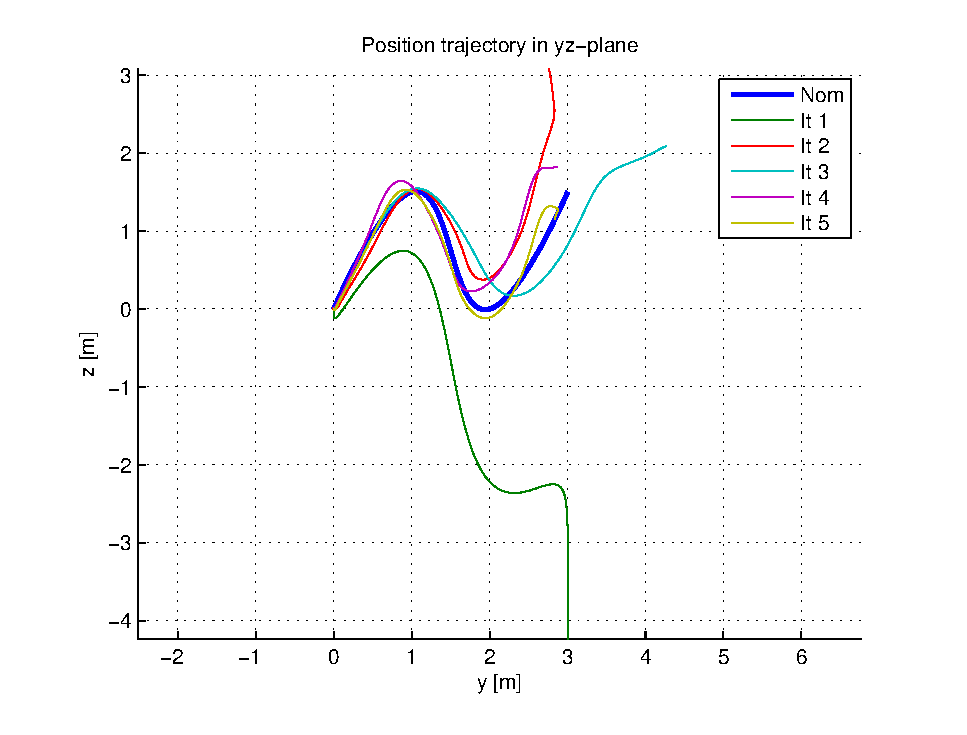
\includegraphics[scale=0.50]{ILCgravity_yz.eps}	
\caption{Tracking results for ILC under gravity mismatch}
\label{fig:ilc_x1}
\end{figure}

Figure \ref{fig:ilc_x1} shows the convergence of the trajectory over iterations. Note that adding more noise reduces the performance, i.e. ILC requires more iterations to converge.

\begin{figure}
\center
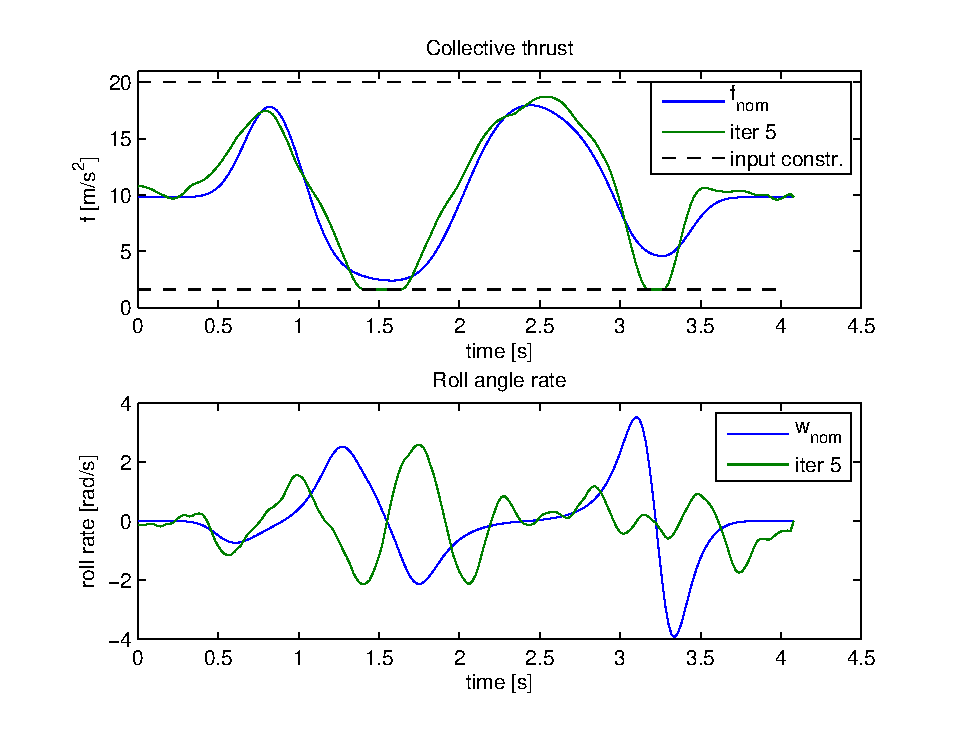
\includegraphics[scale=0.50]{ILCgravity_us.eps}	
\caption{Control inputs over ILC iterations}
\label{fig:ilc_u1}
\end{figure}

Figure \ref{fig:ilc_u1} shows the change in the control inputs needed to accommodate the gravity mismatch. Only the final input is shown, for better visibility.

%CGP-UCB results
Figures \ref{fig:res1_g} - \ref{fig:res2_g}, CGP-UCB learning results again for the same system dynamics. It is assumed here that the cost difference to be learned, as a function of $x := (\context;\sysInput)$, is a realization (or a drawn sample) of a GP with:

\begin{align}
f(x) &\sim \mathcal{N}(\mu(x), k(x, x')) \label{GP prior for quadrocopter} \\
\mu(x) &= 0 %\beta_{\mu}\context + \beta_0 
\label{mean hyperparameters for quadrocopter} \\
k(x, x') &= \sigma_{s}^{2}k_u(\sysInput, \sysInput')k_c(\context, \context') + \sigma_{n}^{2}\delta_{xx'} \label{kernel} \\ 
k_u(\sysInput, \sysInput') &= \sysInput^{\mathrm{T}}\Lambda_{u}^{-2}\sysInput' \label{action kernel} \\
k_c(\context, \context') &= \exp(-\frac{1}{2}(\context-\context')^{\mathrm{T}}\Lambda_{c}^{-2}(\context-\context')) \label{context kernel}
\end{align}

Diagonal matrices $\Lambda_{u}$ and $\Lambda_{c}$ transform anisotropic coordinates into isotropic coordinates or they can be motivated from Automatic Relevance Determination (ARD) point of view where $\Lambda_{u}^{2}$ and $\Lambda_{c}^{2}$ encode the relevance of inputs and contexts, respectively \cite{GPbook}.
This means that hyperparameter estimation is performed with a model structure consisting of 
%a linear mean with intercept and 
a composite kernel that is the product of a linear ARD kernel for the input space $\mathrm{U(t)}$ and a Squared Exponential (SE) ARD kernel for the context space $\mathrm{C}$. For quadrocopter dynamics (\ref{quadrocopterDynamics}) this transforms the problem into a QP-program, see section \ref{ControlAffine}.

\begin{figure}
\center	
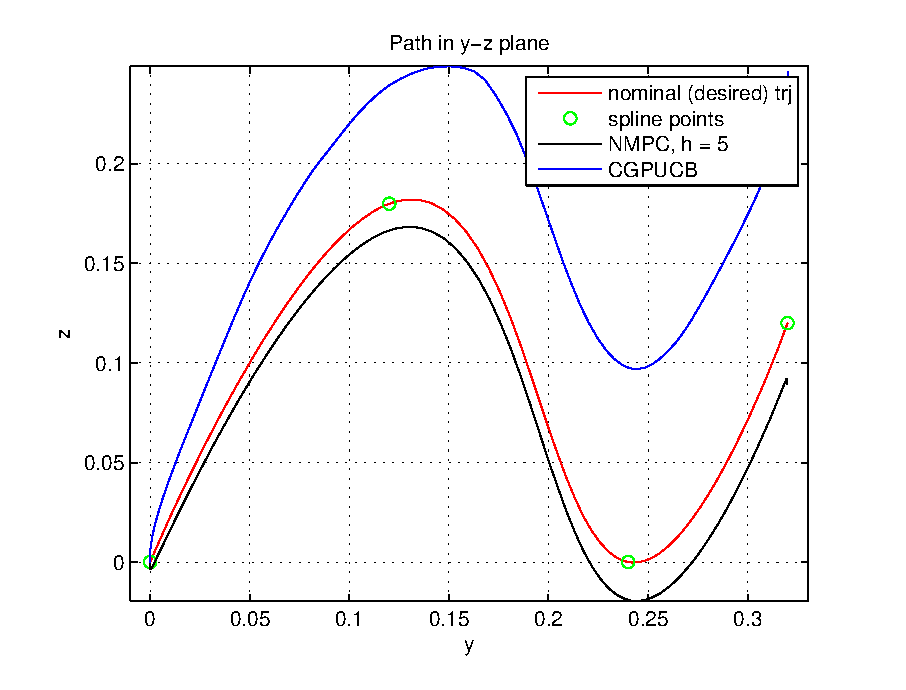
\includegraphics[scale=0.40]{res1_g.eps}	
\caption{Gravity mismatch: tracking results of the first run}
\label{fig:res1_g}
\end{figure}

\begin{figure}
\center
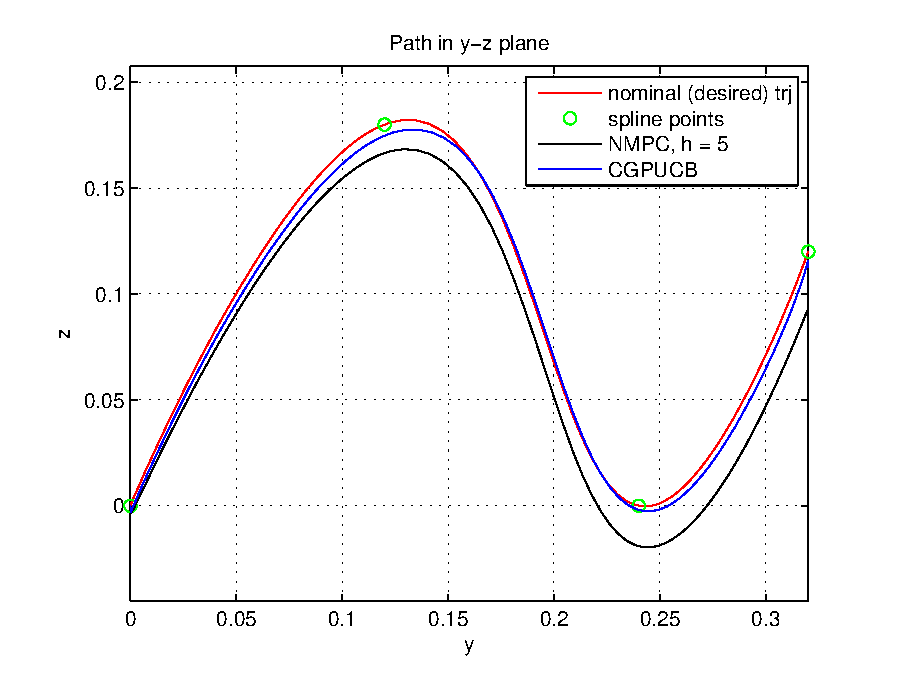
\includegraphics[scale=0.40]{res2_g.eps}	
\caption{Gravity mismatch: tracking results of the third run}
\label{fig:res2_g}
\end{figure}

\begin{figure}
\center
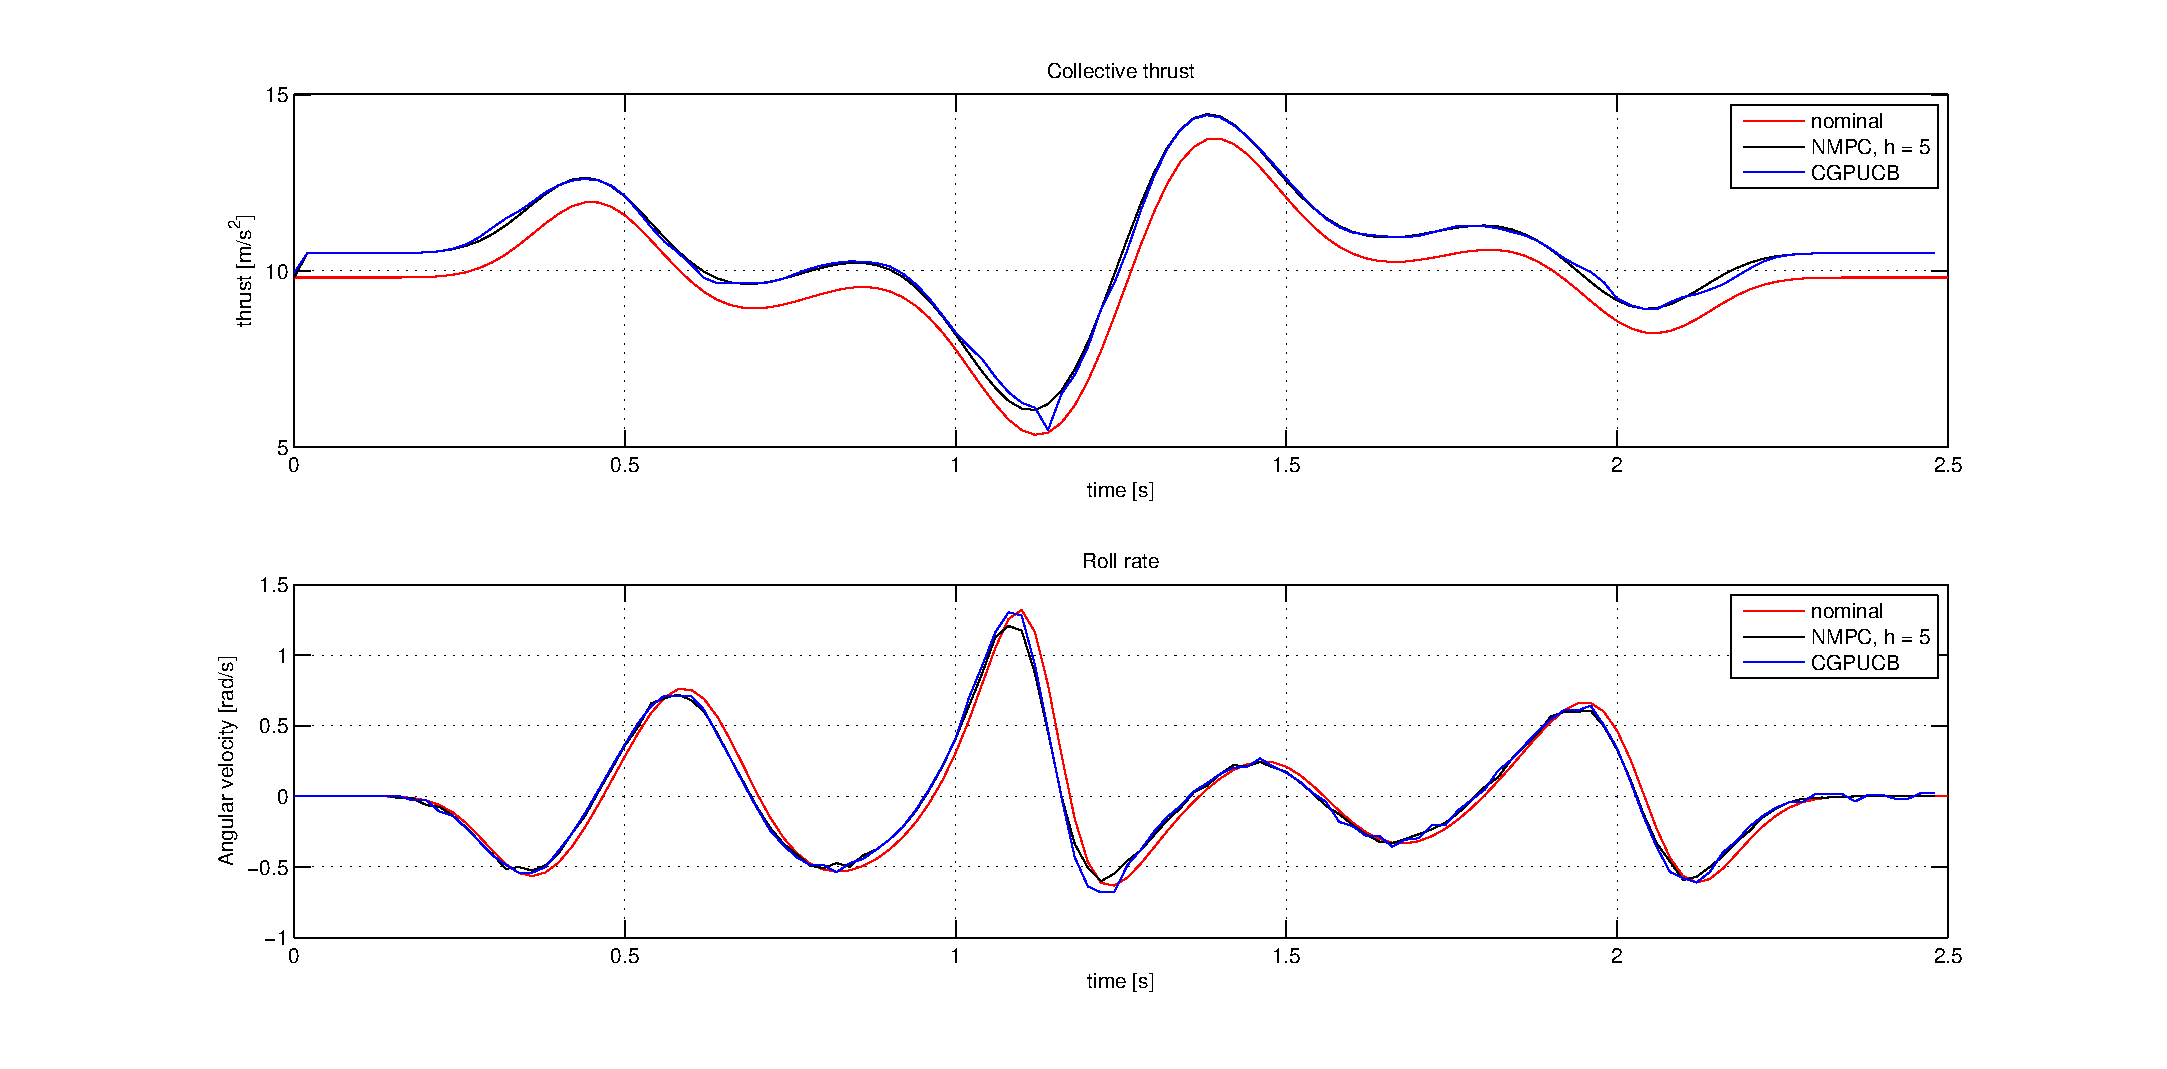
\includegraphics[scale=0.20]{inp1_g.eps}			
\caption{Gravity mismatch: control inputs for the third run}
\label{fig:inp1_g}
\end{figure}

Figure \ref{fig:inp1_g} shows the applied control signals for the third run shown in figure \ref{fig:res2_g}. Sum of squares (SSE) error for the three trials are shown in \ref{SSE_errors}. They clearly show that the method can outperform MPC when disturbances in the form of unknown dynamics are present. $Q$ matrix was taken to be diagonal, with entries $(1,1,1,1,0.01)$.

\begin{table}[h!t]
% increase table row spacing, adjust to taste
\renewcommand{\arraystretch}{1.3}
\caption{SSE errors}
\label{SSE_errors}
\centering
\begin{tabular}{cc}
\textbf{Method / Iteration No.} & SSE \\
\hline
MPC, horizon = 5 & 0.042284 \\
CGP-UCB, trial 1 & 0.914764 \\
CGP-UCB, trial 2 & 0.003622 \\
CGP-UCB, trial 3 & 0.001949 
\end{tabular}
\end{table}

\subsection{Wind Disturbance}
In the second case, we consider a constant horizontal wind force with $P_{wind} = 50 \mathrm{N/m}^{2}$ and $A = 0.16 \mathrm{m}^2$ whose dynamics is analyzed in Example 2, \eqref{example2General}. The cost function difference is given explicitly in equation \eqref{QuadTheta0}. ILC is unable to compensate for this type of disturbance dynamics, as can be seen in Figure \ref{fig:ilc_x2}. 

\begin{figure}
\center	
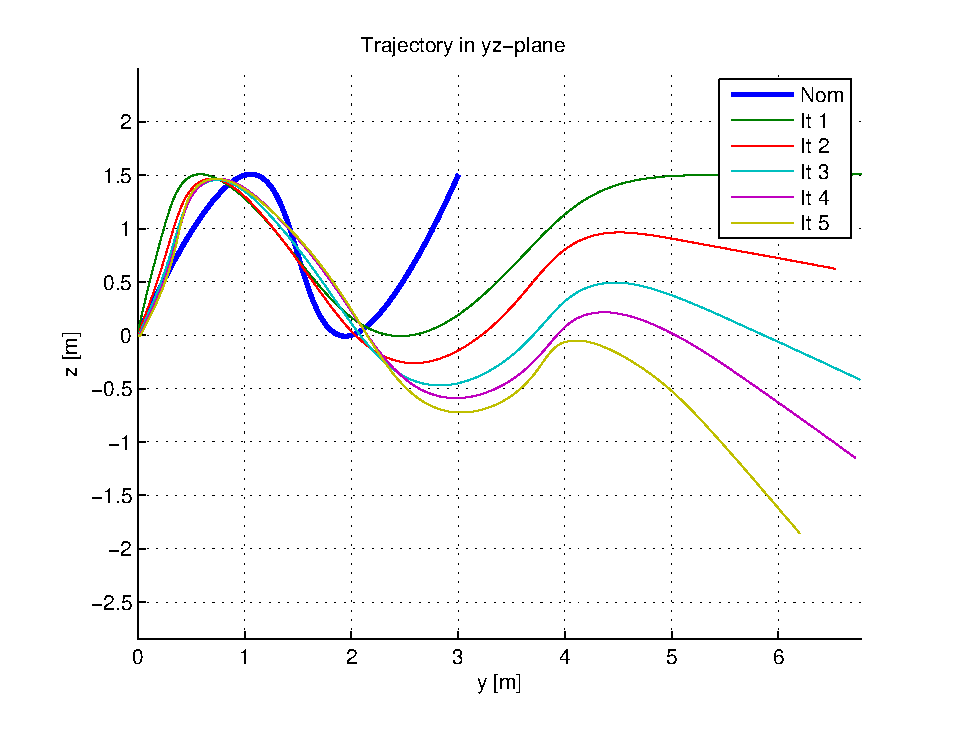
\includegraphics[scale=0.40]{ILCwind_yz.eps}	
\caption{Tracking results for ILC under wind disturbance}
\label{fig:ilc_x2}
\end{figure}

Here transfer learning is shown to take place between two different trajectories. Figure \ref{fig:res1_wind} shows the tracking result for the first trajectory at first iteration. In the second iteration, the trajectory is rotated by 90 degrees. Figure \ref{fig:res2_wind} shows the tracking results for this second trajectory. Comparing with an alternative initial run of the wave trajectory, shown in Figure \ref{fig:res3_wind}, we can clearly see knowledge transfer taking place. This has been accomplished by transferring the costs learned during the first trajectory runs to the second trajectory, using the smoothing provided by the squared exponential kernel for the contexts. However, showing convergence while doing transfer learning over different trajectories, especially in the case of big disturbances, is difficult. There are also issues complicating the application of this approach to transfer learning:

1. The $Q$ matrix. $Q$ was taken to be diagonal with entries $(1,0,0,0,0.01)$. Notice that the variations in the fifth state $\theta$ are only penalized by $0.01$. This causes the applied $w_{x}$ inputs to be very non-smooth. However this lowering of the $\theta$ penalty is necessary to secure learning to track the trajectory with a \emph{single} stage cost. Rolling out the learned cost (stage cost mean) over a horizon should help to make the applied inputs more smooth.

2. Matrix inversion. It takes more trials in general, to show transfer learning, than to show convergence for a single trajectory. But as trials increase, it takes much more time to invert (or use backlash on) the covariance matrix. Reduced rank approximations of the covariance matrix can be applied to speed up the inversion. Mining the past data for \emph{relevant} contexts and inputs then, is a critical part of showing transfer learning.

3. Converging trajectories. Aside from ensuring stability, constructing converging trajectories around the trajectory can help to increase knowledge transfer. By generating trajectories offline perhaps, or perhaps by guiding the process online, one can try to improve the speed of transfer learning. This is because by following the state space around a trajectory, learning can become much more robust to changes in the objective, i.e. the trajectory itself. For the simulations shown in this section, implementing a converging trajectory method $H$, can help to produce better results.

\begin{figure}
\center	
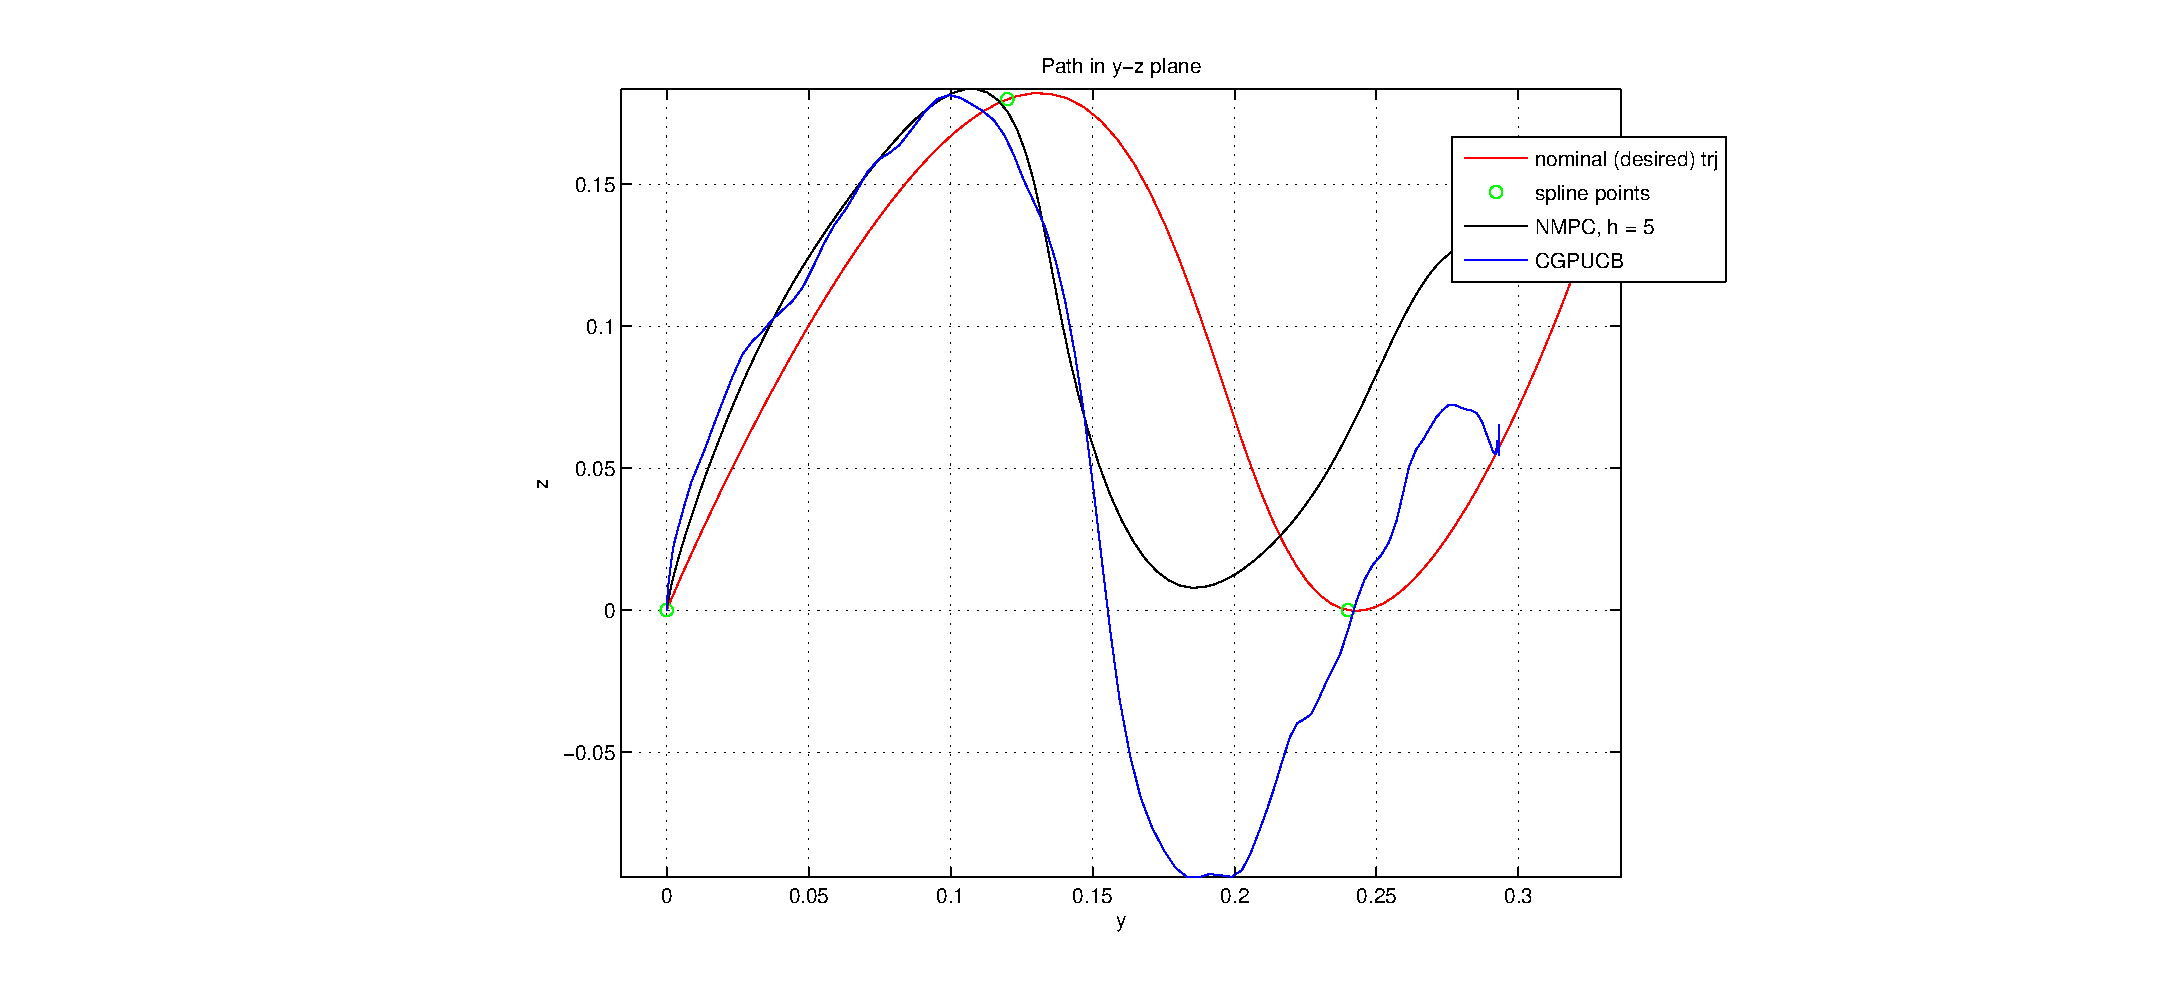
\includegraphics[scale=0.40]{res1_wind.eps}	
\caption{Tracking result of the first trajectory}
\label{fig:res1_wind}
\end{figure}

\begin{figure}
\center
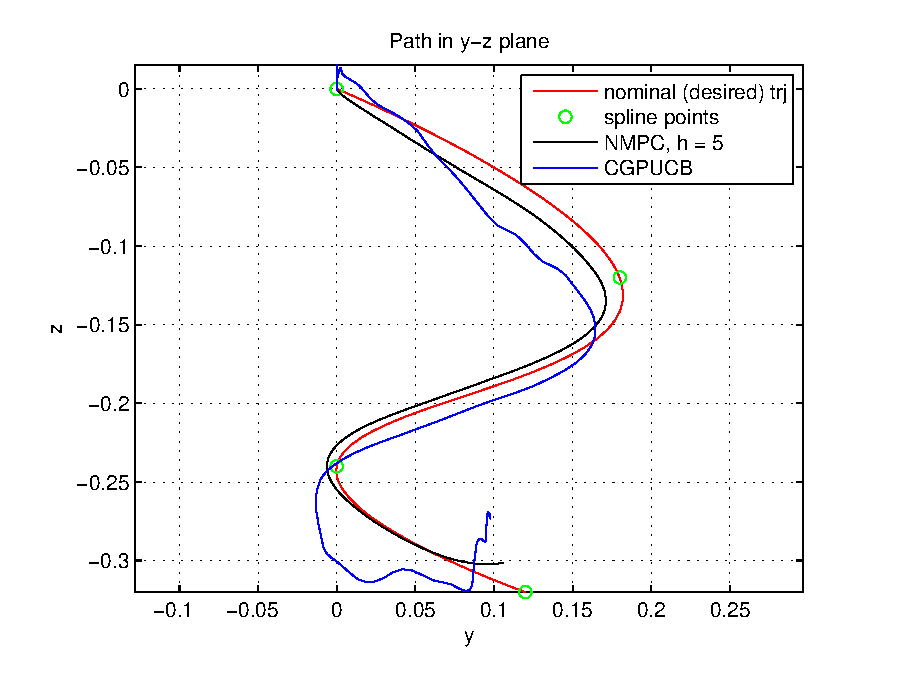
\includegraphics[scale=0.40]{res2_wind.eps}	
\caption{Tracking result of the second trajectory}
\label{fig:res2_wind}
\end{figure}

\begin{figure}
\center
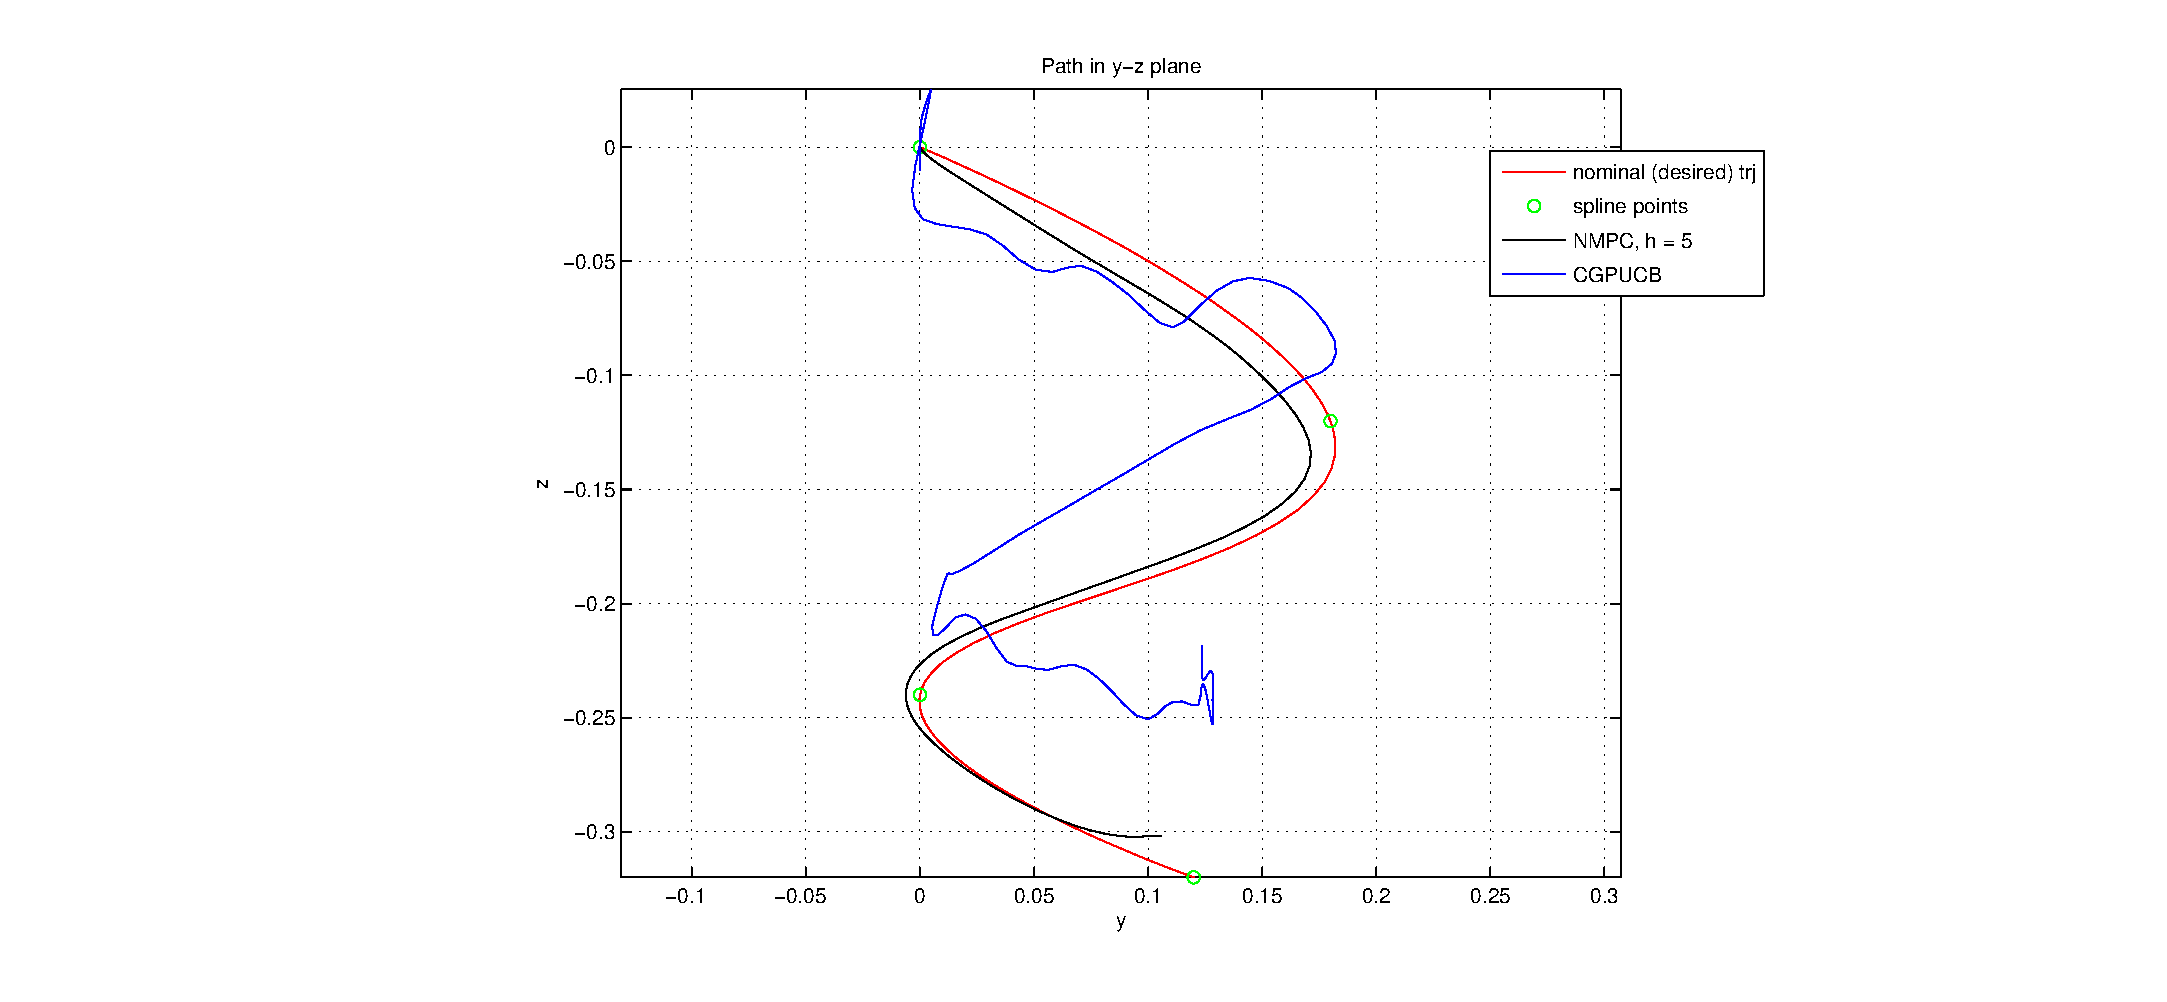
\includegraphics[scale=0.40]{res0_wind.eps}	
\caption{Alternative initial run of the second trajectory}
\label{fig:res3_wind}
\end{figure}
%%\include{Chapter...}
\chapter{Summary}
\label{s:Summary}
%Summarize the presented work. Why is it useful to the research field or institute?

In this thesis, an intuitive upper-confidence style algorithm based on Gaussian Process optimization (CGP-UCB) is implemented on trajectory tracking for control systems where an unknown disturbance dynamics is present. Such dynamics, if severe, can prevent more conventional methods such as Model Predictive Control or Iterative Learning Control from tracking the trajectory. This algorithm learns over trajectories, real time, the stage cost of the partially unknown system dynamics. It works by sub-optimally solving the exploration-exploitation dilemma: it \emph{explores} new control inputs when the uncertainty of that input is high enough, and it \emph{exploits} the learned dynamics (the mean value) as it gets more and more sure of the disturbance dynamics of the system. 

The algorithm was for the first time presented in \cite{Krause1} and then extended to the contextual case in \cite{Krause2}. In Chapter \ref{Introduction}, we reviewed Gaussian Processes and then described the contextual bandits in \ref{ContextBandit}. In Chapter \ref{Chapter1}, we started by reviewing ILC and after mentioning ILC's limitations, we presented the proposed method in \ref{methodology}. In the results section \ref{Results1} some results have been presented where we show learning take place. It is also shown that a significant amount of knowledge can be transferred even between cases where the reference trajectories are not the same. As long as the disturbance dynamics is smooth enough over the state space, the contextual framework helps to transfer knowledge over different trajectories.

The sublinear regret proofs presented in \cite{Krause1} and \cite{Krause2} hold only when the hyperparameters of the GP from which the function to be optimized is drawn, is completely known. In reality, of course, this assumption is not realistic. We have shown in Chapter \ref{Chapter2}, how estimation of hyperparameters can be performed using Maximum Likelihood Estimation (ML). The author is currently unaware of results that hold under parametric mismatch, a point that deserves to be studied more in the literature.

\section{Discussion}

\section{Future Work}
\label{ss:FutureWork}

We believe that investigating this issue could yield new insights on GP optimization and is one of many possible ways to extend the work. Adaptive Hyperparameter Estimation, where hyperparameters can be adapted over different trial runs using particle filter-like methods are of ongoing concern. An initial attempt at such a method has been presented in \cite{Ginsbourger} where they keep a \emph{benchmark of experts}, a set of weighted different hyperparameter models and values. Alternatively, pursuing Bayesian methods for hyperparameter estimation, such as MCMC for the integral given in (\ref{evidence}) might be useful.

In Appendix \ref{app:code} it can be observed that the Restricted Maximum Likelihood (REML) estimates for hyperparameters are not much different from ML estimates. Hence it was concluded in Chapter \ref{Chapter2} that mean parameter estimation might be altogether avoided. However more work needs to be done in order to assert this claim conclusively. 

On the control side, stability and robustness of the proposed method are critical for a safe implementation. Proposition \ref{Prop:1} assumes the existence of a method $H$ that can effectively generate converging trajectories, i.e. with sublinear regret. The construction of $H$ is an important open problem. Perhaps it can be computed offline with Dynamic Programming by discretizing the state space. Or as suggested at the end of \ref{stability}, it can be cast as variance minimization at each step, and implemented if sufficient online computational resources are available. However, such a method, even if it can be explicitly constructed, will only be effective probabilistically. If implemented on a test-bed, an additional layer of safety has to be provided, as in the ILC method presented in \ref{ILC}, that will shutdown the operation if the deviation over the desired trajectory is above the safety limits, or perhaps trigger a more-conservative control method that will bring the operation to a safe halt. Over time, such a fail-safe method (along with $H$) will be needed less and less, as the dynamics is learned. Then, the learned stage cost can be rolled-out over a fixed horizon as in Model Predictive Control (MPC), to make the system more stable under constraints and new disturbances.

%Possible ways to extend the work.
% Extending covariance structure by considering Matern or even Exponential Distribution
% Optimization related issues
% Perturbation analysis
% REML related extensions 

%%%%%%%%%%%%%%%%%%%%%%%%%%%%%%%%%%%%%%%%%%%%%%%%%
%%% Bibliography                              %%%
%%%%%%%%%%%%%%%%%%%%%%%%%%%%%%%%%%%%%%%%%%%%%%%%%
\addtocontents{toc}{\vspace{.5\baselineskip}}
\cleardoublepage
\phantomsection
\addcontentsline{toc}{chapter}{\protect\numberline{}{Bibliography}}
\bibliography{myReferences}
%% All books from our library (SfS) are already in a BiBTeX file
%% (Assbib). You can use Assbib combined with your personal BiBTeX file:
%% \bibliography{Myreferences,Assbib}. Of course, this will only work on
%% the computers at SfS, unless you copy the Assbib file 
%%  --> /u/sfs/bib/Assbib.bib

%%%%%%%%%%%%%%%%%%%%%%%%%%%%%%%%%%%%%%%%%%%%%%%%% 
%%% Appendices (if needed)                    %%%
%%%%%%%%%%%%%%%%%%%%%%%%%%%%%%%%%%%%%%%%%%%%%%%%%
\addtocontents{toc}{\vspace{.5\baselineskip}}
\appendix
\include{Appendix1}
\chapter{Mathematical Identities}\label{app:math}

\section{Incremental Covariance Matrix Inverse}
% note the speedup expected
% In MATLAB backslash is optimized so speedup not observed.

The GP-update equations \eqref{gpUpdate_mu} and \eqref{gpUpdate_sigma}, require the inversion of the matrix $P_{t} \defeq K(x_{T}, x_{T}) + \sigma_{n}^{2}\mathbf{I}$. Since the CPG-UCB optimization \eqref{ucb} requires $\mu(x)$ and $\sigma(x)$ at each time step $t$, this matrix needs to be inverted at each step. The backlash operation to bypass this inversion requires $N^{3}/6$ complexity. For a single test point $x_{t}$, a workaround is to use incremental inverse for the growing matrix:

\begin{equation}
P_{t+1} = 
\left(
\begin{BMAT}(rc){c:c}{c:c}
P_{t} & k(x_{T}, x_{t}) \\
k(x_{T}, x_{t})^{\mathrm{T}} & k(x_{t}, x_{t})
\end{BMAT} 
\right)
\label{CovMat}
\end{equation}

where $k(x_{T}, x_{t}) \defeq (k(x_{1}, x_{t}), \ldots, k(x_{t-1}, x_{t	}))^{\mathrm{T}}$. 

The inverse of a general invertible $n \times n$ partitioned matrix 

\begin{equation*}
A = 
\left(
\begin{array}{cc}
P & Q \\
R & S \\
\end{array} 
\right)
\end{equation*}

is the $A^{-1}$ matrix:

\begin{equation*}
A^{-1} = 
\left(
\begin{array}{cc}
\tilde{P} & \tilde{Q} \\
\tilde{R} & \tilde{S} \\
\end{array} 
\right)
\end{equation*}

where the submatrices are given as \cite{GPbook}:

\begin{eqnarray}
\tilde{P} & = & P^{-1} + P^{-1}QMRP^{-1} \label{Phat}\\
\tilde{Q} & = & -P^{-1}QM \label{Qhat} \\
\tilde{R} & = & -MRP^{-1} \label{Rhat} \\
\tilde{S} & = & M \label{Shat}
\end{eqnarray}

and $M = (S - RP^{-1}Q)^{-1}$. Applying \eqref{Phat} - \eqref{Shat} on the inverse of the covariance matrix \eqref{CovMat} we get:

\begin{equation}
P_{t+1}^{-1} = 
\left(
\begin{BMAT}(rc){c:c}{c:c}
P_{t}^{-1} + \alpha P_{t}^{-1} q_{t} q_{t}^{\mathrm{T}} P_{t}^{-1}  & -\alpha P_{t}^{-1} q_{t} \\
-\alpha q_{t}^{\mathrm{T}} P_{t}^{-1} & \alpha
\end{BMAT} 
\right)
\label{CovMatInv}
\end{equation}

where 

\begin{eqnarray}
\alpha^{-1} & = & k(x_{t}, x_{t}) - q_{t}^{\mathrm{T}}P_{t}^{-1}q_{t} + \sigma_{n}^{2} \\
q_{t} & = & k(x_{t}, x_{T})
\end{eqnarray}

$\alpha$ is a scalar that is the outcome of the last point taken, $x_{t}$. \eqref{CovMatInv} can be reached easily by plugging the block matrices in \eqref{Phat} - \eqref{Shat} and noting that the covariance matrix $P_{t}$ is square symmetric.

A practical way to iteratively compute \eqref{CovMatInv} from $P_{t}^{-1}$ would be to compute first the vector of covariances $q_{t}$  and then $q_{t}^{\mathrm{T}}P_{t}^{-1}$, and apply it throughout the block matrices in \eqref{CovMatInv}. Figure \ref{fig:runtimes} shows the results for such an implementation in MATLAB running on Intel i7 1.6 GHz Quadcore laptop, where the runtimes for the matrix multiplication operation, $(K(x_{T}, x_{T}) + \sigma_{n}^{2}\mathbf{I})^{-1}\mathbf{k}_N(x^{*})$ is compared. The incremental matrix inversion is clearly faster, especially as the data sample size $N$ increases. Figure \ref{fig:deltaruntimes} shows the effect more clearly. Note that for the backslash method, the covariance matrix is not built from scratch at each iteration, but only the last row and column are added.

\begin{figure}
\center
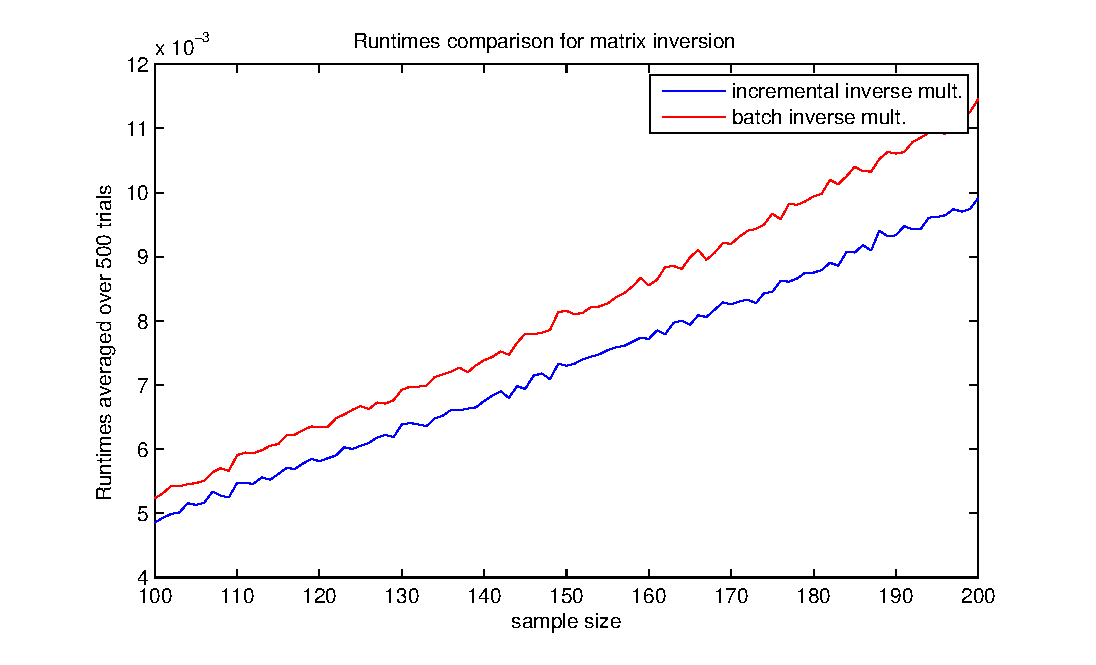
\includegraphics[scale=0.50]{runningtimes.eps}	
\caption{Runtime comparison}
\label{fig:runtimes}
\end{figure}

\begin{figure}
\center
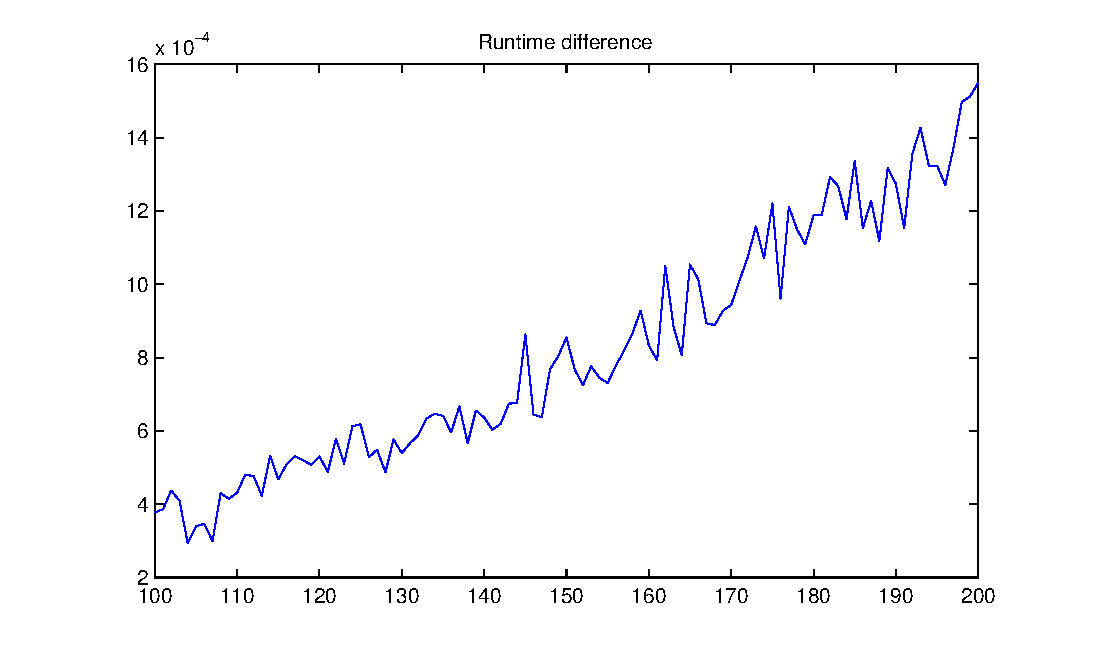
\includegraphics[scale=0.50]{delta_runningtimes.eps}	
\caption{Difference in runtimes}
\label{fig:deltaruntimes}
\end{figure}



%% Epilogue (optional)
\addtocontents{toc}{\vspace{.5\baselineskip}}
\cleardoublepage
\phantomsection
\addcontentsline{toc}{chapter}{\protect\numberline{}{Epilogue}}
\markboth{Epilogue}{Epilogue}
\include{Epilogue}

\end{document}
